\PassOptionsToPackage{unicode}{hyperref}
\PassOptionsToPackage{naturalnames}{hyperref}
\documentclass[a4paper,
               bibliography=totoc,
%                draft=true,
               hidelinks,
               listof=totoc,
               twoside]{scrreprt}
\usepackage[bottom = 3 cm]{geometry}
\usepackage[
  %automark,
  %autooneside=false,% <- needed if you want to use \leftmark and \rightmark in a onesided document
  headsepline %line below header
]{scrlayer-scrpage}
%adds page numbers to center of foot on first chapter page
%\deftripstyle{ChapterStyle}{}{}{}{}{\pagemark}{}
%\renewcommand*{\chapterpagestyle}{ChapterStyle}
%deletes default footer page numbers
\clearpairofpagestyles
%customize header
\ihead{\leftmark}
\ohead{\ifstr{\leftmark}{\rightbotmark}{}{\rightbotmark}}
\lehead{\pagemark}
%right-handed even page headers
\rehead{\headmark}
\lohead{\headmark}
\rohead{\pagemark}
%add section title to header
\automark[section]{chapter}

\usepackage[main=english, ngerman]{babel}
\usepackage[utf8]{inputenc}
\usepackage[T1]{fontenc}
\usepackage{microtype}
\usepackage[onehalfspacing]{setspace}
\usepackage{pdfpages}
\usepackage{lipsum}
\usepackage{etoolbox}
\usepackage{chemformula}
\usepackage{simpler-wick}
\usepackage{listings}
\usepackage{bbold}
\usepackage{physics}
\usepackage{amsmath}
\usepackage{bm}

\clubpenalty10000
\widowpenalty10000

\usepackage[perpage, symbol*]{footmisc}

% uncomment if you want to start next chapter on same page
% \usepackage{etoolbox}
% \makeatletter
% \patchcmd{\scr@startchapter}{\if@openright\cleardoublepage\else\clearpage\fi}{}{}{}
% \makeatother

%for enumeration environment used for own publication list
\usepackage[inline]{enumitem}
  \setlist[itemize]{itemsep=10pt, label={--}}

\usepackage{graphicx}
\usepackage[labelfont=bf, labelsep=space, format=plain]{caption}

%for tabular for appended publications
\usepackage{array}
  \newcolumntype{T}{>{\ttfamily}l}
%   \newcolumntype{L}[1]{>{\raggedright\let\newline\\\arraybackslash\hspace{0pt}  }m{#1}}
  \newcolumntype{L}[1]{>{\raggedright\setlength{\parindent}{-0.3cm}\let\newline\\\arraybackslash\hspace{0pt}}m{#1}}


\usepackage{hyperref} %has to be loaded before glossaries package for hyperlinks of acronyms to work!
\usepackage[acronym, toc, nopostdot]{glossaries}
\usepackage{glossary-longbooktabs}
  \newcommand*\myglsfirst[1]{\glsfirst{#1}\glsunset{#1}}
  \newcommand*\myglsfirstplural[1]{\glsfirstplural{#1}\glsunset{#1}}
  \renewcommand*\glspostdescription{\hfill}
\usepackage{glossaries-prefix}
\newacronym{cc-pV$X$Z}{cc-pV$X$Z}{correlation-consistent polarised valence with $X$-zeta quality ($X$=D, T, Q, 5, 6, ...)}
\newacronym{aug-cc-pV$X$Z}{cc-pV$X$Z}{correlation-consistent polarised valence with $X$-zeta quality ($X$=D, T, Q, 5, 6, ...) augmented with diffuse functions}
\newacronym{cc-pCV$X$Z}{cc-pV$X$Z}{correlation-consistent polarised valence with $X$-zeta quality ($X$=D, T, Q, 5, 6, ...) with core correlation}
\newacronym{ECG}{ECG}{Explicitly Correlated Gaussian}
\newacronym{GTG}{GTG}{Gaussian-type Geminal}
\newacronym{MC}{MC}{Monte Carlo}
\newacronym{API}{API}{application programming interface}
\newacronym{SI}{SI}{supporting information}
\newacronym{DTN}{DTN}{Drummond-Towler-Needs}
\newacronym{MAE}{MAE}{mean absolute error}
\newacronym{MAD}{MAD}{mean absolute deviation}
\newacronym{RMSD}{RMSD}{root mean squared deviation}
\newacronym{MD}{MD}{mean deviation}
\newacronym{MaxD}{MaxD}{maximum deviation}
\newacronym{DF}{DF}{density fitting}
\newacronym{RI}{RI}{resolution of identity}
\newacronym{DIIS}{DIIS}{direct inversion of the iterative subspace}
\newacronym{ITF}{ITF}{integrated tensor framework}
\newacronym{CTF}{CTF}{cyclops tensor framework}
\newacronym{CT}{CT}{charge transfer}
\newacronym{QC}{QC}{quantum chemistry}
\newacronym{BOA}{BOA}{Born-Oppenheimer approximation}
\newacronym{SE}{SE}{Schrödinger equation}
\newacronym{STO}{STO}{Slater-type orbital}
\newacronym{GTO}{GTO}{Gaussian-type orbital}
\newacronym{AO}{AO}{atomic orbital}
\newacronym{MO}{MO}{molecular orbital}
\newacronym{LCAO}{LCAO}{linear combination of atomic orbitals}
\newacronym{SALC}{SALC}{symmetry adapted linear combination}
% \newacronym{vdz}{\textsc{vdz}}{cc-pVDZ}
% \newacronym{avdz}{\textsc{avdz}}{aug-cc-pVDZ}
% \newacronym{vtz}{\textsc{vtz}}{cc-pVTZ}
% \newacronym{avtz}{\textsc{avtz}}{aug-cc-pVTZ}
\newacronym{CBS}{CBS}{complete basis set}
\newacronym{OBS}{OBS}{orbital basis set}
\newacronym{ABS}{ABS}{auxiliary basis set}
\newacronym{CABS}{CABS}{complementary auxiliary basis set}
\newacronym{BSSE}{BSSE}{basis set superposition error}
\newacronym{BSIE}{BSIE}{basis set incompleteness error}
\newacronym{CSF}{CSF}{configuration state function}
\newacronym{SD}{SD}{Slater determinant}
\newacronym{OSS}{OSS}{open-shell singlet}
\newacronym{SCF}{SCF}{self consistent field}
\newacronym{HF}{HF}{Hartree-Fock}
\newacronym{RHF}{RHF}{restricted Hartree-Fock}
\newacronym{ROHF}{ROHF}{restricted open-shell Hartree-Fock}
\newacronym{UHF}{UHF}{unrestricted Hartree-Fock}
\newacronym{QRHF}{QRHF}{quasi restricted Hartree-Fock}
\newacronym{KS}{KS}{Kohn-Sham}
\newacronym{DFT}{DFT}{density functional theory}
\newacronym{TD}{TD}{time dependant}
\newacronym{CAS}{CAS}{complete active space}
\newacronym{IAS}{IAS}{incomplete active space}
\newacronym{MCSCF}{MCSCF}{multiconfigurational self-consistent field}
\newacronym{CASSCF}{CASSCF}{complete active space self-consistent field}
\newacronym{QMC}{QMC}{quantum Monte Carlo}
\newacronym{VMC}{VMC}{variational Monte Carlo}
\newacronym{DMC}{DMC}{diffusion Monte Carlo}
\newacronym{PT}{PT}{perturbation theory}
\newacronym{MP2}{MP2}{second-order M{\o}ller-Plesset perturbation theory}
\newacronym{BCH}{BCH}{Baker-Campbell-Hausdorff}
\newacronym{SR}{SR}{single reference}
\newacronym{MR}{MR}{multireference}
\newacronym{HS}{HS}{Hilbert space}
\newacronym{FS}{FS}{Fock space}
\newacronym{SU}{SU}{state universal}
\newacronym{SS}{SS}{state specific}
\newacronym{DSRG}{DSRG}{driven similarity renormalization group}
\newacronym{ic}{ic}{internally contracted}
\newacronym{CC}{CC}{coupled cluster}
\newacronym{CCD}{CCD}{coupled cluster with double excitations}
\newacronym{CCSD}{CCSD}{coupled cluster with single and double excitations}
\newacronym{CCSD(T)}{CCSD(T)}{coupled cluster with single and double excitations and perturbative triples}
\newacronym{CCSDT}{CCSDT}{coupled cluster with single, double and triple excitations}
\newacronym{CCSDTQ}{CCSDTQ}{coupled cluster up to quadruple excitations}
\newacronym{DC}{DC}{distinguishable cluster}
\newacronym{DCD}{DCD}{distinguishable cluster with double excitations}
\newacronym{DCSD}{DCSD}{distinguishable cluster with single and double excitations}
\newacronym{2D}{2D}{two determinant}
\newacronym{DC-CCSDT}{DC-CCSDT}{distinguishable cluster with single, double and triple excitations}
\newacronym{EOM}{EOM}{equation of motion}
\newacronym{SF}{SF}{spin flip}
\newacronym{LR}{LR}{linear response}
\newacronym{FR}{FR}{fixed reference}
\newacronym{CI}{CI}{configuration interaction}
\newacronym{sCI}{sCI}{selected configuration interaction}
\newacronym{exFCI}{exFCI}{extrapolated selected configuration interaction of \gls{FCI} quality}
\newacronym{exSHCI}{exSHCI}{extrapolated semi-stochastic heat bath configuration interaction}
\newacronym{HEAT}{HEAT}{high-accuracy extrapolated ab initio thermochemistry}
\newacronym[first={MRCI}]{MRCI}{MRCI}{multireference configuration interaction}
\newacronym{ED}{ED}{exact diagonalization}
\newacronym{FCI}{FCI}{full configuration interaction}
\newacronym{FCIQMC}{FCIQMC}{full configuration interaction quantum Monte Carlo}
\newacronym{DMRG}{DMRG}{density matrix renormalization group}
\newacronym{TC}{TC}{transcorrelation}
\newacronym{xTC}{xTC}{transcorrelation via exclusion of explicit three-body components}
\newacronym{FROGG}{FROGG}{frozen Gaussian geminal}
\newacronym{TMM}{TMM}{trimethylenemethane}
% \newacronym{RDM}{RDM}{reduced density matrix}
\newacronym{1RDM}{1RDM}{1-electron reduced density matrix}
\newacronym{2RDM}{2RDM}{2-electron reduced density matrix}
\newacronym{CASPT2}{CASPT2}{complete active space perturbation theory to second order}
\newacronym{MPI}{MPI}{Message Passing Interface}
\newacronym{SA}{SA}{state-averaged}

\makeglossaries

%print Contents also in TOC
\BeforeTOCHead[toc]{\cleardoublepage\pdfbookmark{\contentsname}{toc}}
\KOMAoptions{parskip=false}% no parskip in ToC
\RedeclareSectionCommand[afterskip=1sp minus 1sp]{chapter}% no skip after ToC title
\DeclareTOCStyleEntry[beforeskip=.3cm]{chapter}{chapter}

%make binding margin on first page on left side and not on right
\let\tmp\oddsidemargin
\let\oddsidemargin\evensidemargin
\let\evensidemargin\tmp
\reversemarginpar

\usepackage[
  backend=biber,
  doi=false,
  giveninits=false,
  isbn=false,
  url=false,
  articletitle=true,
  chaptertitle=true,
  style=chem-acs,
  maxbibnames=99,
  maxcitenames=99,
  urldate=iso,
  seconds=true
]{biblatex}

%make title in bib hyperlink to doi
\newbibmacro{string+doi}[1]{%
  \iffieldundef{doi}{#1}{\href{https://doi.org/\thefield{doi}}{#1}}}
\DeclareFieldFormat{title}{\usebibmacro{string+doi}{\mkbibemph{#1}}}
\DeclareFieldFormat[article]{title}{\usebibmacro{string+doi}{\mkbibquote{#1}}}

\usepackage{csquotes}
\DeclareFieldFormat{title}{\textit{#1}}
\DeclareFieldFormat{booktitle}{\textit{#1}}
\DeclareFieldFormat{journaltitle}{\upshape{#1}}
\DeclareFieldFormat{citetitle}{#1}

% add bib files like so -- make sure to keep categorised!
% \addbibresource{./library/[...].bib}
% \addbibresource{library/mypapers.bib}
% \addbibresource{library/*.bib}


\addbibresource{library/Textbooks.bib}
\addbibresource{library/Benchmarks.bib}
\addbibresource{library/F12.bib}
\addbibresource{library/FCIQMC.bib}
\addbibresource{library/H chain.bib}
\addbibresource{library/Misc.bib}
\addbibresource{library/mypapers.bib}
\addbibresource{library/N2.bib}
\addbibresource{library/Sign Problem.bib}
\addbibresource{library/Software.bib}
\addbibresource{library/TC-General-Resurgence.bib}
\addbibresource{library/Textbooks.bib}

\let\cite\supercite

%for onlinecite
\DeclareCiteCommand{\citenum}
  {}
  {\bibhyperref{\printfield{labelnumber}}}
  {}
  {}

\makeatletter
  \newrobustcmd*{\setmaxcitenames}{\numdef\blx@maxcitenames}
\makeatother

%define thesis title etc.

% meta-data variables
\newcommand*{\thetitle}{%
  Development of the Transcorrelated Full Configuration Interaction Quantum Monte Carlo Method
}

\newcommand*{\theapproval}{%
  Von der Fakultät Chemie der Universität Stuttgart zur Erlangung der Würde eines
    Doktors der Naturwissenschaften (Dr.\@ rer.\@ nat.\@) genehmigte Abhandlung
}
\newcommand*{\theauthor}{Jacobus Philip Haupt}
\newcommand*{\thebirthplace}{George, S\"udafrika}
\newcommand*{\thedefensedate}{30 April 2025}
\newcommand*{\thedate}{30 April 2025}
\newcommand*{\theyear}{2025}
\newcommand*{\theuniversity}{Universität Stuttgart}
\newcommand*{\theinstitute}{Max-Planck-Institut für Festkörperforschung, Stuttgart}
\newcommand*{\theadvisor}{Prof.\@ Dr.\@ Ali Alavi}
\newcommand*{\theexamineri}{Prof.\@ Dr.\@ Andreas Köhn}
\newcommand*{\theexaminerii}{Prof.\@ Dr.\@ Joris van Slageren}

%define custom commands
\newcommand{\onlinecite}[1]{Ref.~\citenum{#1}}
\newcommand{\onlinecites}[2]{Refs.~\citenum{#1}, \citenum{#2}}
\newcommand{\onlinecitess}[3]{Refs.~\citenum{#1}, \citenum{#2}, \citenum{#3}}
\newcommand{\todo}[1]{{\color{red}TODO: #1}}
\newcommand*\ownref[1]{Ref.~\textbf{\ref{#1}}}
\newcommand*\superownref[1]{\textsuperscript{\textbf{\ref{#1}}}}
\newcommand{\eq}[1]{Eq.~(\ref{#1})}
\newcommand{\eqs}[2]{Eqs.~(\ref{#1},~\ref{#2})}
\newcommand{\chap}[1]{chapter~\ref{#1}}
\newcommand{\sect}[1]{sec.~\ref{#1}}
\newcommand{\fig}[1]{Figure~\ref{#1}}
\newcommand{\tab}[1]{Table~\ref{#1}}
\newcommand{\NL}{\nonumber \\}
\newcommand{\nl}{\nonumber \\ & }

\newcommand{\mathdef}{\mathrel{\mathop:}=}
\newcommand{\e}{\mathrm{e}}

\newcommand{\red}[1]{{\color{red} #1}}
\newcommand{\blue}[1]{{\color{blue} #1}}
\newcommand{\magenta}[1]{{\color{magenta} #1}}
\newcommand{\brown}[1]{{\color{brown} #1}}
\definecolor{pinegreen}{rgb}{0.0, 0.47, 0.44}
\newcommand{\green}[1]{{\color{pinegreen} #1}}

\newcommand{\molpro}{\textsc{molpro} }
\newcommand{\casino}{\textsc{casino} }
\newcommand{\pyscf}{\textsc{pyscf} }
\newcommand{\tchint}{\textsc{tchint} }
\newcommand{\pytchint}{\textsc{pytchint} }
\newcommand{\github}{GitHub }
\newcommand{\quantumpackage}{\textsc{quantum package} }
\newcommand{\dice}{\textsc{dice} }
\newcommand{\quest}{\textsc{quest} }
\newcommand{\elemcojl}{\textsf{ElemCo.jl} }
\newcommand{\quantwo}{\textsf{Quantwo} }
\newcommand{\ccdiag}{\textsc{ccdiag} }
\newcommand{\wicked}{\textsc{Wick}\&\textsc{d} }
\newcommand{\pdgq}{\texttt{p$^\dg$q} }

\newcommand{\hartree}{$E_\mathrm{h}$}
\newcommand{\Ms}{M_\mathrm{s}}
\newcommand{\ac}[1]{\ensuremath{a_{#1}^\dagger}}
\newcommand{\ad}[1]{\ensuremath{a_{#1}}}
\newcommand{\el}{}

\newcommand{\mat}{\mathbf}
% \newcommand{\op}[1]{\hat{\mathrm{#1}}}
\newcommand{\dg}{\dagger}
\newcommand{\half}{\frac{1}{2}}
\newcommand{\third}{\frac{1}{3}}
\newcommand{\quart}{\frac{1}{4}}
% \DeclareMathOperator\erf{erf}
% Define \lt and \gt for `less than' and `greater than'
\mathchardef\lt="313C \mathchardef\gt="313E
% Set up `<' and `>' as angle brackets
\mathcode`<="4268 \mathcode`>="5269
% \newcommand{\bra}{{\texttt bra }}
% \newcommand{\ket}{{\texttt ket }}
%\newcommand{\Perm}[2]{{\cal P}\left(#1,#2\right)}
\newcommand{\Perm}[2]{\hat{\cal P}^{#1}_{#2}}
\newcommand{\sop}[1]{{\cal S}\left(#1\right)}
\newcommand{\Sop}[2]{{\cal S}\left(#1,#2\right)}
\newcommand{\asop}[1]{{\cal A}\left(#1\right)}
\newcommand{\ASop}[2]{{\cal A}\left(#1;#2\right)}
\newcommand{\spa}[1]{{#1}}
\newcommand{\spb}[1]{\bar{#1}}

\newcommand{\one}{\mathbb{1}}

% for presubscripts and presuperscripts (e.g., \pre{^x}U_a)
\newcommand{\pre}[1]{\,#1\!}

\DeclareUnicodeCharacter{3B1}{\ensuremath{\alpha}}
\DeclareUnicodeCharacter{3B2}{\ensuremath{\beta}}
\DeclareUnicodeCharacter{3B3}{\ensuremath{\gamma}}
\DeclareUnicodeCharacter{3B4}{\ensuremath{\delta}}



%https://tex.stackexchange.com/questions/246411/koma-script-how-to-style-the-title-of-a-chapter
\KOMAoption{chapterprefix}{true}
\renewcommand*\raggedchapter{\centering}
\newif\ifmakeupper
\newcommand*\chaptertitleformat[1]{\ifmakeupper\MakeUppercase{#1}\else#1\fi}
\addtokomafont{chapter}{\makeuppertrue}
\setkomafont{chapterprefix}{\normalsize\mdseries}
\renewcommand*{\chapterformat}{%
    \MakeUppercase{\chapappifchapterprefix{\nobreakspace}}\thechapter\autodot%
    \IfUsePrefixLine{%
      \par\nobreak\vspace{-\parskip}\vspace{-.6\baselineskip}%
      \rule{0.9\textwidth}{.5pt}%
    }{\enskip}%
}
\RedeclareSectionCommand[beforeskip=0pt,afterskip=4\baselineskip]{chapter}

\renewcaptionname{english}{\contentsname}{\chaptertitleformat{Contents}}

\begin{document}

\pagenumbering{roman}
\begin{titlepage}
  \begin{spacing}{1}
    \begin{center}
      \begin{otherlanguage}{ngerman}
        % no indentation of paragraphs
        \setlength{\parindent}{0pt}

        ~\vspace{1em}

        {\bfseries\huge\thetitle\par}

        \vfill

        \theapproval

        \vfill

        Vorgelegt von

        {\bfseries\Large\theauthor\par}

        aus \thebirthplace

        \vfill

        \begin{tabular}{ll}
          Hauptberichter:   &\theadvisor\\
          Mitberichter:     &\theexamineri\\
          Prüfungsvorsitzender: &\theexaminerii\\
          \multicolumn{2}{l}{%
            Tag der mündlichen Prüfung:\quad%
            \thedefensedate%
          }
        \end{tabular}

        \vfill

        
\includegraphics[width=60mm]{./figures/logos/CI_MPI_FKF_MPG_gruen.pdf}
        \hspace{1em}
        
\includegraphics[width=60mm]{./figures/logos/logoUniversity}

        \vspace{2em}

        \theuniversity{}

        \vspace{1em}

        \theinstitute{}

        \vspace{1em}

        \theyear
      \end{otherlanguage}
    \end{center}
  \end{spacing}
\end{titlepage}
\cleardoublepage


% don't display page number
\thispagestyle{empty}

\vspace*{\fill}

\begin{minipage}{0.865\textwidth}%
  \begin{center}
    \begin{minipage}{0.80\textwidth}%
      \begin{flushleft}
        \textit{%
          It is important to realize that in physics today, we have no knowledge of what energy \emph{is}.
        }
      \end{flushleft}
      \begin{flushleft}
        \small--- Richard Feynman, \textit{Feynman Lectures on Physics, Volume 1, Chapter 4}
      \end{flushleft}
    \end{minipage}%
  \end{center}
\end{minipage}

\vspace*{\fill}

\cleardoublepage

% \setcounter{tocdepth}{1}
\tableofcontents
\cleardoublepage


\begin{otherlanguage}{ngerman}
\addchap{Erklärung über die Eigenständigkeit der Dissertation}

Ich erkläre hiermit an Eides statt, dass ich die vorliegende Arbeit
  \begin{quote}
    \glqq{}\textit{\thetitle{}}\grqq{}
  \end{quote}
  ohne Hilfe Dritter und ohne Benutzung anderer als der angegebenen
    Hilfsmittel angefertigt habe; die aus fremden Quellen direkt oder
    indirekt übernommenen Gedanken sind als solche kenntlich gemacht.
  Die Arbeit wurde bisher in gleicher oder ähnlicher Form in keiner anderen
    Prüfungsbehörde vorgelegt.
\end{otherlanguage}


\vspace{4cm}

\noindent\rule{5cm}{.4pt}\hfill\rule{5cm}{.4pt}\par
\noindent Datum, Ort \hfill Unterschrift

\addchap{Acknowledgements}

Foremost, I would like to thank my supervisor \textbf{Ali Alavi} for his guidance and undying optimism, as well as for being an excellent professional role model. Similarly, I would like to thank \textbf{Daniel Kats} for his professional guidance and patience with me as I learned the basics of electronic structure theory, especially at the start of my PhD while I was still working remotely from Vancouver. \textbf{Nikolay Bogdanov} has also been extremely helpful in guiding me with active-space methods. I also extend a thanks to my committee members \textbf{Joris van Slageren} and \textbf{Andreas K\"ohn}.

Similarly, much of my professional development can be owed to mentors along the way, in particular \textbf{Darryl Barber}, \textbf{Christian Ast}, and \textbf{Roman Krems}.

I also thank \textbf{Evelin Christlmaier} for all her support, both professionally and personally, and with whom working has been a pleasure.While our time together in the group was short, \textbf{Werner Dobrautz} distilled in me a greater sense of mindfulness and reassurance that everything will be okay. Similarly, \textbf{Johannes Hauskrecht} has been a wonderful officemate with whom I could always whine about life as a PhD student.

My time at MPI has, to my pleasure, involved a lot of software development, and for that I am especially grateful to have had such knowledgeable coworkers as \textbf{Robert Anderson} and \textbf{Oskar Weser} to go to for advice and with whom to argue which text editor is best.

I would also like to thank my former and present coworkers \textbf{Pablo L\'opez R\'ios}, \textbf{Aron Cohen} and \textbf{Kai Guther} for their work on making \tchint a reality. \textbf{Andreea Filip}, \textbf{Kristoffer Simula} and \textbf{Ke Liao} have been especially pivotal in making the \pytchint package possible.

Navigating administration as a foreigner in Germany can be extremely difficult, but this stress has been lifted off my shoulders by \textbf{Birgit King}, to whom I am much in debt.

% \todo{Friends back home: Karan(!), Michael, Charlie, Zack, Cam, Mr Barber}

Finally, I want to thank my dear friends who made my time in Stuttgart infinitely more colourful: \textbf{Aybike Reyhanl\i}, \textbf{Thomas Schraivogel}, \textbf{Ingemar Schmidt}, \textbf{Rut Martinez}, \textbf{Nikos Papanikolaou}, \textbf{Aim\'ee Sousa Calepso}, \textbf{Martin Baumann}, and especially \textbf{Theresa Huber} with whom I shall always cherish our countless hours dancing together.

\printglossary[type=\acronymtype]
% \printglossary[type=\acronymtype, nonumberlist]
%\printglossary[title={Symbols}, style=long-booktabs, nonumberlist]

\cleardoublepage
\begin{otherlanguage}{ngerman}
\addchap{Zusammenfassung}

Die Transkorrelierte (TC) Methode ist eine Methode in der Quantenchemie, die in den letzten Jahren an Bedeutung gewonnen hat. In dieser Methode wird eine Ähnlichkeitstransformation auf den elektronischen Hamiltonoperator angewandt, um Korrelationseffekte, insbesondere die dynamische Korrelation, durch explizite Behandlung analytisch bekannter Eigenschaften des Hamiltonoperators zu erfassen. Diese Methode wurde bereits mit der ,,Full Configuration Interaction Quantum Monte Carlo'' (FCIQMC) Methode kombiniert, einer effizienten stochastischen Methode zur Lösung der Schrödingergleichung und zur Berechnung physikalischer Observablen. Diese Dissertation widmet sich einer vertieften Untersuchung dieser Methoden, insbesondere der TC-Methode.

Nach einer Wiederholung der Grundlagen wellenfunktionsbasierter und Quantum-Monte-Carlo Methoden, wird die Verwendung flexibler Jastrow-Faktoren, die in der Literatur des ,,Variational Quantum Monte Carlos'' (VMC) bekannt sind, vorgestellt. Damit minimieren wir die Varianz der TC-Referenzenergie. Es zeigt sich, dass dies zu einer schnellen Basissatzkonvergenz führt und eine Genauigkeit erreicht, für die herkömmliches FCIQMC viel größere Basissätze erfordern würde. Außerdem kompaktiert dieses Minimierungsverfahren auch die Wellenfunktion, was eine effizientere FCIQMC-Berechnung ermöglicht. Im weiteren Verlauf erweitern wir die Methode für Probleme mit starken Multireferenzcharakter, insbesondere indem wir die Dissoziation des Stickstoffdimers als Stresstest verwenden. Wir zeigen die Notwendigkeit eines Multireferenz-Jastrow-Faktor-Ansatzes auf und minimieren deshalb die Varianz eines Multireferenzzustands. Dies wird nachweislich günstige, größenkonsistente Energien wiederherstellen und gleichzeitig die schnelle Basissatzkonvergenz von TC erreichen. Da nach der Jastrow-Faktor-Optimierung eine Multireferenztechnik (FCIQMC) verwendet wird, erhöht sich der rechnerische Skalierung für die Methode darüber hinaus nicht, wenn man die konventionelle (nicht-TC-)Form derselben Multireferenztechnik wie beim TC-Ansatz verwendet.

Abschließend untersuchen wir die Möglichkeit, vereinfachte Jastrow-Faktoren zu konstruieren, um das bisherige Optimierungsverfahren für die TC-Methode, das rechenintensiv sein kann, zu verbessern oder sogar ganz zu umgehen. Einerseits zeigen wir, dass parameterfreie Jastrow-Faktoren aufgrund der Fehlerkompensation zu schlechten absoluten Energien, aber guten relativen Energien führen können. Andererseits ergeben Jastrow-Faktoren, die für Atome optimiert und für Moleküle wiederverwendet wurden, sowohl genaue absolute als auch relative Energien. Dies eröffnet die Möglichkeit, Jastrow-Faktoren für Atome im gesamten Periodensystem zu optimieren und sie in einer Datenbank zu speichern, die für größere Moleküle abgefragt werden kann, was die Skalierbarkeit der Methode unterstützt.

\end{otherlanguage}

\addchap{Abstract}
The transcorrelated (TC) method is a technique in electronic structure theory that has recently been gaining momentum. In it, a similarity transformation is applied to the electronic Hamiltonian to capture effects of electron correlation, particularly dynamical correlation, by explicit treatment of analytically-known properties of the Hamiltonian near coalescence points. This has already been combined with the full configuration interaction quantum Monte Carlo (FCIQMC) method, an efficient stochastic approach to solving the electronic Schrödinger equation and calculating physical observables. This dissertation further explores these methods, particularly TC.

After a recapitulation of the core concepts of wave function and quantum Monte Carlo methods, we introduce the use of flexible Jastrow factors familiar in the variational Monte Carlo (VMC) literature to minimise the variance of the TC-reference energy. This is shown to result in a rapid basis-set convergence, reaching accuracy for which conventional FCIQMC would require much larger basis sets. Moreover, this minimisation procedure is shown to also compactify the wave function, allowing for more efficient sampling in FCIQMC. We next extend the methodology for problems of strongly multireference character, notably using the dissociation of the nitrogen dimer as a stress test. We illustrate the need for a multireference Jastrow-factor ansatz, and hence minimise the variance of a multireference state. This is shown to recover favourable, size-consistent energies while maintaining the rapid basis-set convergence that comes with TC. As a multireference technique (FCIQMC) is used after optimisation, it moreover does not increase the computational scaling of the method to use the conventional (non-TC) form of the same multireference technique as the TC ansatz.

Finally, we explore the possibility of constructing simplified Jastrow factors in order to improve or possibly wholly bypass the optimisation procedure so far for the TC method, which can be computationally expensive. We show that parameter-free Jastrow factors can result in poor absolute energies, but favourable relative energies thanks to error cancellation, whereas Jastrow factors optimised for atoms and reused for molecules result in both accurate absolute and relative energies. This opens the possibility of optimising Jastrow factors for atoms across the periodic table and storing them in a database, which can be queried for larger molecules, thereby aiding the scalability of the method.


\pagenumbering{arabic}
\setcounter{page}{1}
\glsresetall

% aim for 120-200 pages

% from Ali:
% Normally a thesis will have three original chapters and two or three introductory/theory chapters
% three original chapters (discussed with Ali) would be:
% Optimization paper
% binding curve/size consistency paper
% (py)tchint
% I guess deterministic optimisation can be mentioned in the tchint chapter
% ECPs can be mentioned as an outlook, so can solids
\chapter{Introduction}
\label{chap:intro}

According to modern quantum theory, to fully describe a (nonrelativistic) system of $N_A$ nuclei and $N_e$ electrons, we must solve the time-dependent Schr\"odinger equation,
\begin{equation}
    \label{eq:schrodinger}
    i \hbar \frac{\partial}{\partial t} \Psi(\bm{x}, t)
    = \hat{H} \Psi(\bm{x}, t)
\end{equation}
where $\bm x=(\bm{r}, \sigma)$, $\bm r\in\mathcal{R}^{3(N_e+N_A)}$ gives the spatial coordinates, and $\sigma$ the corresponding spins. For nuclei with atomic numbers $Z_I$ (positive charge $Ze$), the Hamiltonian operator $\hat H$ may be written

\begin{align}
\begin{split}
\label{eq:theory_of_everything}
\hat H =& -\sum_{I=1}^{N_A}\frac{\hbar^2}{2m_I} \nabla^2_I
+ \frac 1{4\pi\epsilon_0} \frac 12\sum_{I,J=1;I\neq J}^{N_A} \frac{Z_IZ_Je^2}{|\bm R_I-\bm R_J|} \\
&- \sum_{i=1}^{N_e} \frac{\hbar^2}{2m_e} \nabla^2_i
+ \frac 1{4\pi\epsilon_0} \frac 12\sum_{i,j=1;i\neq j}^{N_e} \frac{e^2}{|\bm r_i-\bm r_j|}
- \frac 1{4\pi\epsilon_0}\sum_{i=1}^{N_e} \sum_{I=1}^{N_A} \frac{Z_I e^2}{|\bm r_i-\bm R_I|}
\end{split}
\end{align}
where $N_A$ and $N_e$ are the number of nuclei and electrons, respectively, and we have represented the nuclear coordinates by $\bm R_I$ and the electron coordinates by $\bm r_i$.

Since quantum chemistry and condensed matter sciences are in general concerned with nonrelativistic processes involving electrons and nuclei, this might boldly be called the \emph{theory of everything}.\cite{laughlinTheory2000} Hence, we may be tempted to conclude this dissertation early, but in practice the evaluation of the Hamiltonian in equation \ref{eq:theory_of_everything} is impossible. First, there is no closed form solution of equation \ref{eq:schrodinger} with this Hamiltonian. Second, numerical evaluation of $\hat H$ is far from trivial.

Let's consider a simple example, the Argon atom. Say we want to solve this partial differential equation on a grid. Let's choose a very coarse $10\times 10\times 10$ grid. Then \emph{at each time step} we need to store $10^{3\times (18+18)}=10^{108}$ values, corresponding to all the particle positions and the grid. Considering there are ``only'' $\sim 10^{80}$ atoms in the known universe,\cite{rydenIntroduction2017} this is completely unreasonable.

This system has only 18 electrons and 18 nuclei, a far cry from the $10^{23}$ or higher number of electrons in a typical condensed matter system, for example. Moreover, we have not taken into account floating point precision, or that we would need to calculate this for possibly many time steps. Clearly, drastic approximations and more sophisticated methods are required.

\section{Overview of the Thesis}

This dissertation fits into the field of nonrelativistic electronic structure theory, the branch of quantum chemistry concerned with the description of electrons and their correlation inside molecules and materials. More specifically, this dissertation focuses on high-accuracy (but often high-cost) \emph{ab initio} methodologies, especially \gls{FCIQMC} and \gls{TC}. As such, we will only be discussing small systems consisting of only a few atoms, as they are tractible with a full, all-electron treatment with these methods. In principle, these methods should be able to be embedded \cite{jonesEmbedding2020,christlmaierFull2022} into more large-scale calculations using multiscale techniques, but this is outside the scope of my work. Nevertheless, the work herein is focused on methodologies, and not on particular physical systems.

The outline of the dissertation is as thus:
\begin{itemize}
    \item Chapter \ref{chap:intro} (this chapter) provides a basic overview of electronic structure theory methods and some of its principal concepts. Sections \ref{sec:hf} and \ref{sec:post-hf} in particular are largely based on the appropriate chapters of reference \citenum{helgakerMolecular2014}.
    \item Chapter \ref{chap:explicit} reviews the current works in so-called ``explicitly correlated'' methods, notably the well-established R12/F12 and the recently-reinvigorated \gls{TC}.
    \item Chapter \ref{chap:qmc} provides a basic introduction to \gls{QMC} and how it relates to \gls{FCIQMC}.
    \item Chapter \ref{chap:opt} discusses optimization strategies of Jastrow factors in the context of \gls{TC}.
    \item Chapter \ref{chap:binding} discusses an extension of the methods in the previous chapters to ensure size consistency and success when targeting strongly multireference problems.
    \item Chapter \ref{chap:universal} discusses methods for modular and universal Jastrow factor forms.
    \item The final chapter, chapter \ref{chap:sumandout}, provides a review and an outlook for the field.
    \item \autoref{chap:pytchint} provides an overview of the software \pytchint developed in the group for evaluation of \gls{TC} integrals.
\end{itemize}


\section{Principal Approximations}

As discussed, to make any progress in electronic structure theory, we must make use of approximations. Of course, we must always be cautious and suspicious when using these, and make sure they are valid for the systems in question. Thankfully, over the course of the last century, a cornucopia of different approximations has been developed to tackle the Schr\"odinger question, some of which will be discussed in this section.

\subsection{The Born-Oppenheimer Approximation}

The most important approximation used in electronic structure theory is the \gls{BOA}.\cite{bornZur1927} The \gls{BOA} relies on the fact that the nuclei are much heavier than the electrons, with the mass of a single proton being almost 2000 times the mass of an electron. As an intuitive picture, we may think of the nuclei as moving much slower than the electrons, which can adapt themselves to the instantaneous positions of the nuclei. In mathematical terms, this means we can take the total wave function to be a product of its nuclear and electronic components,
\begin{equation}
    \Psi_\mathrm{total} = \Psi_\mathrm{nuc} \Psi_\mathrm{elec}.
\end{equation}

Notice that the first two terms of equation \ref{eq:theory_of_everything} are independent of the electronic coordinates and, ipso facto, have no effect on $\Psi_\mathrm{elec}$. This leads to the \emph{electronic Hamiltonian} under the \gls{BOA}, which can be written as
\begin{equation}
\label{eq:elec_hamiltonian}
\hat H_\mathrm{elec} = -\sum_{i} \frac{1}{2} \nabla_i^2 - \sum_{i,I} \frac{Z_I}{r_{iI}} + \sum_{i\gt j} \frac{1}{r_{ij}},
\end{equation}
where we have simplified notation by using miniscule roman letters for the electrons and capital roman letters for the nuclei, and $r_{ij}=|\mathbf{r}_i-\mathbf{r}_j|$ and $r_{iI}=|\mathbf{r}_i-\mathbf{R}_I|$, as well as by using atomic units. That is, the system of units where $\hbar$, $e$, $m_e$, and $4\pi\epsilon_0$ all correspond to the value of $1$.

In the language of second quantisation, equation \ref{eq:elec_hamiltonian} can be written as
\begin{equation}
\label{eq:elec_hamiltonian_2q}
\hat H_\mathrm{elec} = \sum_\sigma\sum_{pq} h^p_{q}a_{p\sigma}^\dag a_{q\sigma}+\frac 12 \sum_{pqrs} V^{pq}_{rs}a_{p}^\dag a_{r}^\dag a_{s}a_{q},
\end{equation}
where $p,q,r,s$ are general spatial-orbital indices, and $a_{p}$ ($a_{p}^\dag$) is the annihilation (creation) operator for an electron in spatial-orbital $p$. $\sigma,\tau$ are the spin indices. These must obey the anti-commutation relations
\begin{equation}
    \{a_{p},a_{q}^\dag\}
    \mathdef
    a_{p}a_{q}^\dag + a_{p}^\dag a_{q}
    =\delta_{pq}
\end{equation}
\begin{equation}
    \{a_{p},a_{q}\} = \{a_{p}^\dag,a_{q}^\dag\} = 0
\end{equation}
so that the electrons satisfy the Pauli exclusion principle.

In equation \ref{eq:elec_hamiltonian_2q}, $h^p_{q}$ is a one-body integral,
\begin{equation}
\label{eq:hij}
h^p_{q} = \int \mathrm{d}^3r\ \phi_p^*(\mathbf{r})\left(-\frac 12 \nabla^2 - \sum_I \frac{Z_I}{|\mathbf{R}_I-\mathbf r|}\right)\phi_q(\mathbf{r})
\end{equation}
and $V^{pq}_{rs}$ is a two-body integral,
\begin{equation}
    V^{pq}_{rs} = \int \mathrm{d}^3r\int\mathrm{d}^3r'\ \phi_p^*(\mathbf{r})\phi_r^*(\mathbf{r}')\frac{1}{|\mathbf{r}-\mathbf{r}'|}\phi_q(\mathbf{r})\phi_s(\mathbf{r}'),
\end{equation}
with a spatial-orbital basis $\{\phi_i(\mathbf{r})\}$.

For our purposes, we neglect the first term of equation \ref{eq:theory_of_everything}, and treat the second term as approximately constant, so $\hat H_\mathrm{nuc} = \sum_{IJ} Z_IZ_Jr_{IJ}^{-1}$. Thus, we are left with the problem of solving the electronic structure problem, which is the subject of this dissertation. Solving the electronic problem for different nuclear positions gives us the potential energy surface.

Note that while chemists and physicists typically talk about the positions of nuclei in a molecule or solid as if they are fixed in place, as will be done in this dissertation, this is really a colloquialism. If the nuclei had an exact position and zero kinetic energy, the \gls{BOA} would be in direct contradiction of the Heisenberg uncertainty principle. Instead, on the timescale of the electrons, due to the much higher mass of nuclei, in the \gls{BOA} we treat the nuclei as approximately localised in a state in which their motion is much slower than that of the electrons (but, importantly, not zero). This keeps the approximation from being in conflict with the fundamental postulates of quantum theory.

The \gls{BOA} is an immensely practical tool as it substantially simplifies our equations, and in many applications it is an excellent approximation. It will be a fundamental assumption throughout the rest of this dissertation, though it need not always be valid in all of quantum chemistry.

While we have done a lot to drastically reduce the complexity of equation \ref{eq:theory_of_everything}, equation \ref{eq:elec_hamiltonian_2q} is still intractible for large system sizes, scaling combinatorially with the size of the Hilbert space, as a function of the system size $N_e$ (henceforth $N$), and the basis set size $M$. Hence, in addition to using a smaller basis, we still need extra approximations and sophisticated methodologies.


\subsection{Core Orbitals}
\label{sec:core_electrons}

In the ground state of a single atom, electrons first occupy the lowest orbitals. The first occupied shells are typically where the electrons are the most tightly bound.\footnote{This neglects symmetries: energy may be higher due to the angular momentum while staying spatially closer to the nucleus.}

Since they tend to be further from the nucleus in an atom, the valence (non-core) orbitals are typically the most affected by the introduction of additional atoms in the system. It is therefore often the valence orbitals that are most important in chemical systems. For this reason, we sometimes ``freeze'' the core orbitals, meaning they remain doubly occupied by electrons, and only correlate the valence orbitals. It is also common to refer to core electrons and valence electrons, meaning those electrons occupying the core and valence orbital space, respectively (though this is technically imprecise language, as electrons are indistinguishable).

Similarly, we may also delete virtual orbitals, typically those of high energy, to further reduce the size of the problem. The remaining space is known as an active space, and is the basic idea of the \gls{CAS} methods.

\subsection{Model Hamiltonians}

In 1929, the surrealist artist Ren\'e Magritte displayed a now-famous painting of a pipe with the caption \emph{Ceci n'est pas une pipe} (French for ``This is not a pipe''). It was meant to depict the idea that the painting itself is in a way treacherous: it may appear to be a pipe, but you cannot stuff it or smoke from it, as it is a representation of a pipe.

In a similar way, physicists and chemists often use \emph{model Hamiltonians}, which do away with aspects of equation \ref{eq:theory_of_everything} that are not expected to be relevant to the problem at hand, resulting in new Hamiltonians that may be considered a representation of equation \ref{eq:theory_of_everything}, much like Magritte's painting.\footnote{We might further argue that all of science can be described this way, as scientific models are always ``mere'' representations of Nature, and are not Nature itself.} Compared to \emph{ab initio} Hamiltonians like equation \ref{eq:elec_hamiltonian_2q}, model Hamiltonians are generally much simpler, but depend on parameters whose values we may not necessarily know a priori.

The most famous model Hamiltonian is the Hubbard model,\cite{Hubbard1963} most typically used to describe electrons in a periodic lattice, and can be written as
\begin{equation}
\label{eq:hubbard}
\hat H_\mathrm{Hubb} = - \sum_{\langle p,q\rangle}\sum_\sigma t_{pq} a_{q\sigma}^\dag a_{p\sigma} + \sum_p U_p\hat n_{p\uparrow}\hat n_{q\downarrow},
\end{equation}
where $\langle p,q\rangle$ denotes nearest neighbour sites, $t_{pq}$ (often taken to be constant, $t$) is a parameter called the hopping amplitude, and $U_p$ (often taken to be constant, $U$) is a parameter called the on-site repulsion. Here we have used a spatial-orbital basis labels $\{p,q\}$ and spin labels $\sigma\in\{\uparrow,\downarrow\}$. $\hat n_{p\sigma}\mathdef a_{p\sigma}^\dag a_{p\sigma}$ is the number operator.

Despite its apparent simplicity, the Hubbard model is a rich model, and has been used to describe a variety of phenomena, from metal-insulator transitions to high-temperature superconductivity. Moreover, it is not always so simple to solve, and has been the subject of much research.\cite{Lieb1968a,liebermannFCIQMC2023}

Let's consider an especially simple version of the model, with only two sites, and open boundary conditions:
\begin{equation}
\label{eq:hubbard_h2}
\hat H_\mathrm{Hubb} = - t\sum_{\sigma}(a_{1\sigma}^\dag a_{2\sigma} + a_{2\sigma}^\dag a_{1\sigma}) + U(\hat n_{1\uparrow}\hat n_{1\downarrow}+\hat n_{2\uparrow}\hat n_{2\downarrow}).
\end{equation}
We could use this as an approximate description of the H$_2$ molecule, where the electrons are restricted to only the lowest 1s orbitals. Compared to equation \ref{eq:theory_of_everything}, this is a tremendously easy problem now.

Of course, when solving a problem using a model Hamiltonian, we must be careful in choosing the correct one. In particular, the exact solution to the Hubbard model in one dimension\cite{Lieb1968a} does not appear to be in agreement with the \emph{ab initio} solution of a one-dimensional chain of hydrogen atoms.\cite{Motta2017,Motta2020}

\section{The Variational Principle}
\label{sec:variational_principle}

One way of finding approximations to the lowest energy eigenstate of a quantum problem like that of equation \ref{eq:elec_hamiltonian_2q} is the variational method. Several methods discussed in this dissertation build on the variational method, and the variational method itself is based on the variational principle, which states\cite{sakuraiModern2017} for any ``trial wave function'' $\ket{\tilde\Psi}$ and Hermitian operator (such as the electronic Hamiltonian) $\hat H$,
\begin{equation}
    \label{eq:variational_principle}
    \frac{\bra{\tilde\Psi}\hat H\ket{\tilde\Psi}}{\braket{\tilde\Psi}}
    \ge E_0 \mathdef  \frac{\bra{\Psi}\hat H\ket{\Psi}}{\braket{\Psi}}
\end{equation}
where $E_0$ is the lowest eigenvalue (e.g. the ground state energy). That is, the energy of $\ket{\tilde\Psi}$ is an upper bound of the exact energy of the system.

To prove this, consider an expansion of $\ket{\tilde\Psi}$ terms of the exact eigenkets $\ket k$ of $\hat H$, so that $\hat H\ket k = E_k\ket k$ and $\ket{\tilde\Psi}=\sum_kc_k\ket k$. Then
\begin{align}
\label{eq:var_proof}
    \begin{split}
    \frac{\bra{\tilde\Psi}\hat H\ket{\tilde\Psi}}{\braket{\tilde\Psi}}
    &=
    \frac{\sum_{kk'}c_k^*c_{k'}\bra{k}\hat H\ket{k'}}{\sum_{kk'}\bra{k}\ket{k'}c_k^*c_{k'}}\\
    &= \frac{\sum_k|c_k|^2(E_k-E_0)}{\sum_k|c_k|^2} + E_0 \\
    &\ge E_0
\end{split}
\end{align}
where, in going from the first to the second line, we used the orthonormality of the eigenbasis $\{\ket k\}$ and that the left- and right-eigenvectors are the same. That is, we used the fact the $\hat H$ is a Hermitian operator. This is an important observation for future discussions, such as in section \ref{sec:tc}.

\section{The Schr\"odinger Equation as a Matrix Problem}
\label{sec:matrix}

Implicit in the operator algebra of the fermionic creation and annihilation operators $a^\dag$ and $a$ in equation \ref{eq:elec_hamiltonian_2q} is the Pauli exclusion principle: we cannot have two or more fermions occupying identical states. In the context of electronic structure theory and this dissertation, the fermions and states in question are electrons and orbitals, respectively. This handles the antisymmetry requirement of the fermionic wave function, $\hat P_{ij}^\sigma\Psi = -\Psi$, where $\hat P_{ij}^\sigma$ permutes the $i$th and $j$th electrons with spin $\sigma$.

Our wave function can hence be expanded by a linear combination of \glspl{SD},
\begin{equation}
    \label{eq:SD_expansion}
\Psi = \sum_i c_i \ket{D_i},
\quad \text{where } \ket{D_i} =
\frac 1{\sqrt{N!}}\left|
    \begin{matrix}
        \chi_1(\bm x_1) & \chi_1(\bm x_2) & \cdots & \chi_1(\bm x_N)\\
        \chi_2(\bm x_1) & \chi_2(\bm x_2) & \cdots & \chi_2(\bm x_N)\\
        \vdots & \vdots & \ddots & \vdots\\
        \chi_N(\bm x_1) & \chi_N(\bm x_2) & \cdots & \chi_N(\bm x_N)\\
    \end{matrix}
 \right|
\end{equation}
for a spin-orbital basis $\{\chi_p(\bm x_q)\}$. A spin-orbital is typically written as a product of a spatial part and a spin part, e.g. $\chi(\bm x) = \phi(\bm r)\omega(\sigma)$.

Given such a finite spin-orbital basis of size $2M$ ($M$ spatial orbitals with 2 different spins each),\footnote{We assume here the same number of spin-$\uparrow$ and spin-$\downarrow$ orbitals for simplicity, though it need not always be the case.} the \gls{SD} expansion is also finite. Therefore, we may write $\hat H$ as a square matrix and equation \ref{eq:elec_hamiltonian_2q} as an eigenvalue equation,
\begin{equation}
\label{eq:eval_eqn}
\hat H\Psi = E\Psi.
\end{equation}

Note, however, that in order to make this a finite-dimensional matrix eigenvalue problem, we needed to use a finite spin-orbital basis. Thus, $E$ in equation \ref{eq:eval_eqn} is not the true ground state energy of the system, but indeed only an approximation within that basis set. This is the case even if we were to solve equation \ref{eq:eval_eqn} exactly. In order to get the true ground state energy, we need to reach the \gls{CBS}, i.e. $M\to\infty$.

With equation \ref{eq:eval_eqn}, we have transformed the hopelessly intractible partial differential equation \ref{eq:theory_of_everything} into a finite algebraic eigenvalue problem, which is much better suited for solving on a computer.

If we have $N_\uparrow$ spin-up electrons and $N_\downarrow$ spin-down electrons, we then have
\begin{equation}
\label{eq:scaling}
|\mathcal{H}| = {M \choose N_\uparrow}{M\choose N_\downarrow}
\end{equation}
where $|\mathcal{H}|$ denotes the size of the Hilbert space, and we have assumed that the number of spin-up orbitals $M$ is equal to the number of spin-down orbitals. Here, ${n\choose r}=\frac{n!}{r!(n-r)!}$ is a binomial coefficient.

The combinatorial scaling is still unfavourable. For a closed-shell system with 20 electrons in 20 orbitals, $|\mathcal{H}|=3.41\times 10^{10}$. Assuming we wish to have double precision,\footnote{A double precision floating-point number has 1 bit for the sign, 11 bits for the exponent, and 52 bits for digits in the number (known as the mantissa or significand).\cite{ascherFirst2011} This resolves to 64 bits or 8 bytes.} to store the whole matrix we would need about $10^{23}$ bytes, or 100 zettabytes. So, while we've substantially reduced the complexity of the problem, it is still extremely demanding. More approximations are therefore needed.

\subsection{Orbitals}
\label{sec:orbitals}

Orbitals (and spin-orbitals), a term already used in this text, describe the spatial distribution (and in the case of spin-orbitals, also the spin) of a single electron. We assume that spatial orbitals form an orthonormal set, and that they form a complete space for an arbitrary wave function. However, in theory to have a \gls{CBS} would mean needing an infinite number of basis functions. In practice, we must of course have a finite basis, and so this naturally leads to a hierarchy of basis sets, where the typically larger basis sets are both more expensive and more accurate.

Many different basis set families exist, but among the most popular are those due to Dunning and coworkers.\cite{dunningGaussian1989} Additionally, many different basis set extrapolation techniques have also been developed.\cite{fellerEffectiveness2011,halkierBasisset1998,halkierBasisset1999,helgakerBasisset1997,jensenBasis1999,pansiniExtrapolation2016,petersonBenchmark1994,woonBenchmark1994}

Strictly speaking, any kind of set of functions can be used as a basis set, as long as they are a complete set. However, in practice we may broadly categorise them into two groups: \glspl{STO} and \glspl{GTO}.

The exact solution for the Hydrogen atom is the Slater-type function $\frac 1{\sqrt{\pi}} \e^{-r}$, and similarly we know that molecular orbitals also decay as $\sim e^{-\zeta r}$.

However, these \glspl{STO} are difficult to work with, as integrals of the form
\begin{equation}
    \label{eq:two-body-integral}
\int\d^3r_1\int d^3r_2\ \phi_p^*(\bm r_1)\phi_r^*(\bm r_2)\frac 1 {r_{12}}\phi_q(\bm r_1)\phi_s(\bm r_2)
\end{equation}
are routinely needed.

Therefore, \glspl{GTO} have been developed,\cite{boysElectronic1950} which have the form $\e^{-\alpha r^2}$. \glspl{GTO} are much easier to handle, as the product of a gaussian is also a gaussian, and the integral of a gaussian is exactly known, so equations like \ref{eq:two-body-integral} have known solutions. With this comes a tradeoff, since we know \glspl{STO} more faithfully capture the form of molecular orbitals, but \glspl{GTO} are much better suited for computations. For this, the most common basis sets typically use a linear combination (or ``contraction'') of gaussians fitted to a \gls{STO}. An illustration is shown in figure \ref{fig:sto-gto}.

It must be noted, however, that \glspl{STO} and \glspl{GTO} have different asymptotic behaviour for $r\to\infty$ and $r\to 0$. The latter in particular will be discussed in section \ref{sec:cusp}.

\begin{figure}[htbp]
    \centering
    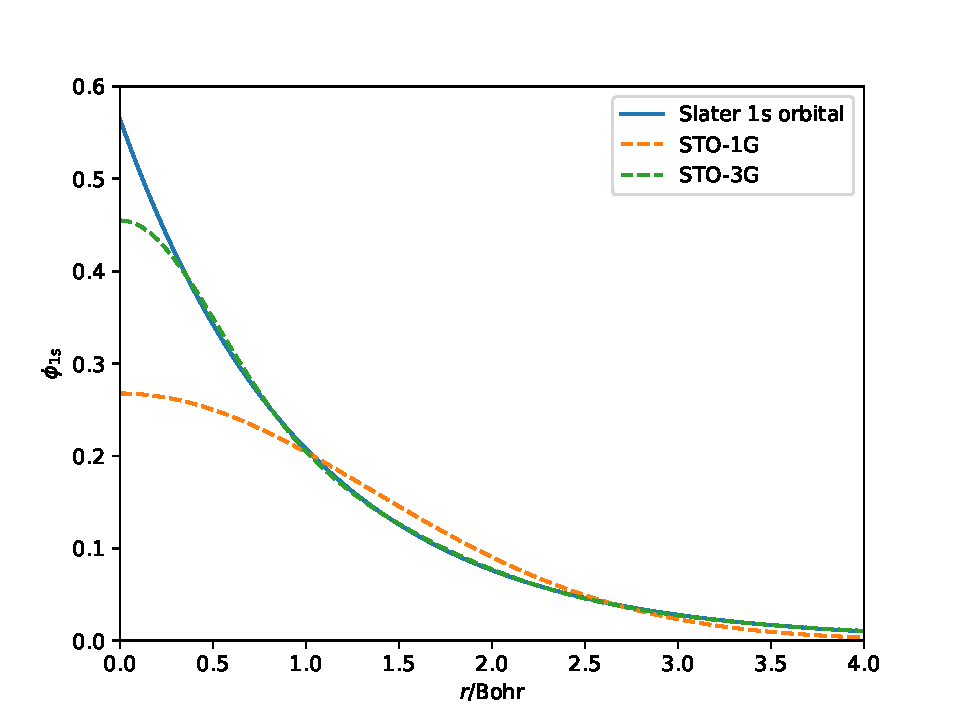
\includegraphics{figures/intro/gto-sto.pdf}
    \caption{Illustration of an $s$-type orbital and the fitted gaussians (STO-$x$G means $x$ gaussians are used to approximate the \gls{STO}). Note that for much of the curve, there is good agreement, but not for the short- and long-range. The short-range behaviour in particular leads to complications, and is the focus of the methods discussed in chapter \ref{chap:explicit}. The long-range behaviour is typically less of a problem, since the integrals we are interested in typically decay with $r$. Fitting parameters for the gaussians were taken from reference \citenum{szaboModern2012}.}
    \label{fig:sto-gto}
\end{figure}

\subsection{Density Matrices}
\label{sec:density-matrices}

The \gls{1RDM} is defined by its matrix elements
\begin{equation}
    \gamma_{pq} = \bra{\Psi}a_q^\dag a_p \ket{\Psi},
\end{equation}
or written in a spin-orbital basis:
\begin{equation}
    \label{eq:one-rdm}
    \gamma(\bm x_1, \bm x_2) = \sum_{pq} \phi_q(\bm x_2)^*\phi_p(\bm x_1) \gamma_{pq}
\end{equation}

Similarly, the \gls{2RDM} is defined as
\begin{equation}
    \label{eq:two-rdm}
    \Gamma_{pqrs} = \bra{\Psi}a_s^\dag a_r^\dag a_q a_p \ket{\Psi}.
\end{equation}

Any one- and two-electron Hermitian operator $\Omega$ can be written (in a spin-orbital basis) as
\begin{equation}
    \label{eq:rdm-expectation}
    \bra{\Psi}\Omega\ket{\Psi} = \sum_{pq} \gamma_{pq}\Omega_{pq} + \sum_{pqrs} \Gamma_{pqrs}\Omega_{rpsq}.
\end{equation}

\subsection{Electron Correlation}
\label{sec:correlation}

% note: primarily using haettig F12 review paper here
Two variables are independent (or uncorrelated) if the joint probability distribution is the product of their expected values, i.e.
\begin{equation}
    P(\bm x_1, \bm x_2) = P(\bm x_1)P(\bm x_2).
\end{equation}

By Bayes' theorem,\cite{hastieElements2009,bayesLII1997} this can be rewritten in terms of the conditional probability,
\begin{equation}
    P(\bm x_1|\bm x_2) = \frac{P(\bm x_1, \bm x_2)}{P(\bm x_2)} = \frac{P(\bm x_1)P(\bm x_2)}{P(\bm x_2)} = P(\bm x_1).
\end{equation}
The variables are said to be correlated if the above is not true.

In the case of electronic structure, the variables in question are $\bm x \mathdef (\bm r, \sigma)$, the spatial coordinates and spin of the electrons. Therefore, when we speak of electron correlation, we are referring to these relations. Furthermore, as electrons are indistinguishable, for every pair $(\bm x_1, \bm x_2)$,
\begin{align}
    &P(\bm x_1) = P(\bm x_2) = \frac 1N \rho(\bm x) \\
    &P(\bm x_1, \bm x_2) = \frac 1{N(N-1)} \rho(\bm x_1, \bm x_2)
\end{align}
where $\rho(\bm x)$ is the electron density and $\rho(\bm x_1, \bm x_2)$ is the probability of finding electrons at $(\bm x_1, \bm x_2)$ simultaneously, known as the pair density,
\begin{align}
    \rho(\bm x) &= N\int \d^3x_2 \cdots \d^3x_N \Psi^*(\bm x, \bm x_2, \bm x_3, \cdots, \bm x_N)\Psi(\bm x, \bm x_2, \bm x_3, \cdots, \bm x_N) \\
    \rho(\bm x_1, \bm x_2) &= N(N-1)\int \d^3x_2 \cdots \d^3x_N \Psi^*(\bm x_1, \bm x_2, \bm x_3, \cdots, \bm x_N)\Psi(\bm x_1, \bm x_2, \bm x_3, \cdots, \bm x_N).
\end{align}

There are two key sources of electron correlation: Fermi correlation, which arises from the fact that electrons obey Fermi statistics, i.e. the wave function is antisymmetric with respect to exchange of $\bm x_1$ and $\bm x_2$, and Coulomb correlation, which arises from the fact that electrons repel each other.

\section{The Hartree-Fock Method}
\label{sec:hf}

The typical starting point to most \emph{ab initio} electronic structure methods is the \gls{HF} method.\cite{hartreeWave1928,fockNaherungsmethode1930,slaterNote1930} The key approximation in \gls{HF} is that we treat the exact $N$-body wave function solution as approximately a single \gls{SD}.\footnote{More precisely, the \gls{HF} approximation is to treat the wave function as a single configuration. In the context of this dissertation, that configuration will always be a \gls{SD}.} Then, we variationally (see section \ref{sec:variational_principle}) optimise the energy of the system with respect to parameters pertaining to the spin-orbitals. We will refer to this \gls{SD} as $\ket{\Phi_0}$.

Then, for some arbitrary initial configuration $\ket 0$,
\begin{equation}
\ket{\Phi_0} = \e^{-\kappa} \ket 0.
\end{equation}
Here,
\begin{equation}
\kappa = \sum_{pq} \kappa_{pq}a_p^\dag a_q
\end{equation}
is an anti-Hermitian operator (i.e. $\kappa_{pq}^* = -\kappa_{qp}$) whose matrix elements $\kappa_{pq}$ are the orbital rotation coefficients and will be the variational parameters. The anti-Hermiticity of $\kappa$ ensures that the orbital rotation $\e^{-\kappa}$ is unitary.

With $\braket{\Phi_0}=1$, we want
\begin{equation}
E_\mathrm{HF} = \min_{\kappa_{pq}}\bra{\Phi_0}\hat H\ket{\Phi_0}.
\end{equation}
This is a nonlinear equation, and hence the parameters $\kappa_{pq}$ must be determined iteratively. Since $\e^{-\kappa}$ is unitary, the orthonormality of the spin-orbitals is preserved, $\bra{\phi_p}\ket{\phi_q} = \delta_{pq}$.

The \gls{HF} method can also be understood as a mean-field theory. That is, we treat the $N$-body problem as $N$ one-body problems, where a single electron is in an effective ``averaged'' potential from the other $N-1$ electrons. This effective one-body Hamiltonian is known as the Fock operator,
\begin{equation}
    \label{eq:fock-operator}
    f = \sum_{pq} f^p_{q} a_p^\dag a_q.
\end{equation}

The Fock operator $f$ may be written as
\begin{equation}
    f = h + V_\mathrm{eff}
\end{equation}
where the Fock potential's matrix elements are $V_{\mathrm{eff},pq}=\sum_{i\in\mathrm{occ}}(V^{pq}_{ii}-V^{pi}_{iq})$.

The Hartree-Fock orbitals, which ultimately dictate the parameters for the minimisation procedure, are determined by diagonalising the Fock matrix,
\begin{equation}
    f^p_{q} = \epsilon_p\delta^p_{q}
\end{equation}
where the eigenvalues $\epsilon_p$ are known as the orbital energies.

Since $f$ itself depends on the orbitals, the solution must be determined self-consistently. Hence \gls{HF} is often referred to as a \gls{SCF} method.

Often, the orbitals for the $\uparrow$ and $\downarrow$ electrons are restricted to be the same. This is known as the \gls{RHF} method. Otherwise, we might instead use the \gls{UHF} method, where they are treated independently. However, since this breaks spin symmetry, we might have spin contamination. \Gls{ROHF} is a variant that can treat open-shell systems which \gls{RHF} otherwise would not be able to treat while remaining an eigenstate of the $S^2$ (total spin) operator.

\subsection{Correlation Energy}

The correlation energy (for a given basis set) is defined as the difference between the exact energy and the \gls{HF} energy,
\begin{equation}
E_\mathrm{corr} = E_\mathrm{exact} - E_\mathrm{HF}.
\end{equation}
It should be noted, however, that despite this name the \gls{HF} method captures Pauli exchange, and hence does actually correlate electrons. Nevertheless, we typically neglect this when we speak of ``correlation energy''.

Similarly, the Coulomb hole is defined as the remaining part of the wave function that is not captured by the \gls{HF} method,
\begin{equation}
    \Psi_\mathrm{hole} = \Psi_\mathrm{exact} - \Psi_\mathrm{HF}.
\end{equation}

\subsection{The Roothaan-Hall Equations}

The Roothaan-Hall equations are a matrix representation of the \gls{HF} approximation.\cite{roothaanNew1951,hallMolecular1997} Given a basis set, typically \glspl{GTO}, the Roothaan-Hall equations are given by the generalised eigenvalue problem,
\begin{equation}
    FC = SC\bm\epsilon
\end{equation}
where $C$ is a matrix of coefficients, $F$ is the Fock matrix (which depends on $C$), $S$ is the overlap matrix (which reduces to the identity matrix for orthonormalised bases), and $\bm\epsilon$ is a diagonal matrix of orbital energies. The Roothaan-Hall equations are obtained by expanding the unknown \glspl{MO} in a basis of known functions, typically \glspl{AO}.

Since this representation is in matrix form, instead of in terms of derivatives and integrals, it is more amenable to conventional computational techniques.

\section{Post-Hartree-Fock Methods}
\label{sec:post-hf}

While the \gls{HF} method is convenient and can be used efficiently to solve for many electrons, it is oftentimes not sufficient to describe the electronic structure of a molecule. To account for the remaining correlation, numerous post-Hartree-Fock methods (that is, methods run after \gls{HF}) have been formulated, some of which are described in this section.

Correlation energy is typically categorised as either dynamical or static, although their effects are not mutually exclusive and so sometimes the distinction can be hazy.

Dynamical correlation is remaining correlation that arises due to the instantaneous repulsion from the motion (dynamics) of the electrons.

Static correlation, on the other hand, is related to the degeneracy or near-degeneracy of configurations. In general, to accurately describe a system with strong static correlation, a so-called multi-reference method is needed. As will be seen in chapter \ref{chap:binding}, static correlation plays a big role for molecules at dissociation.

We therefore have two ``axes'' on which to approach the exact solution to equation \ref{eq:elec_hamiltonian_2q}:
\begin{itemize}
    \item The basis set chosen, where going to a larger basis set (in a systematic way) improves the result, e.g. cc-pVDZ to cc-pVTZ to cc-pVQZ, until eventually reaching the \gls{CBS} limit.
    \item The ``hierarchy of theories'' where the more accurate the method, the closer to the \gls{FCI} limit (discussed below). Many post-Hartree-Fock methods can be systematically improved, for example by considering additional excitations in a coupled cluster method.
\end{itemize}

\begin{figure}[htbp]
    \centering
    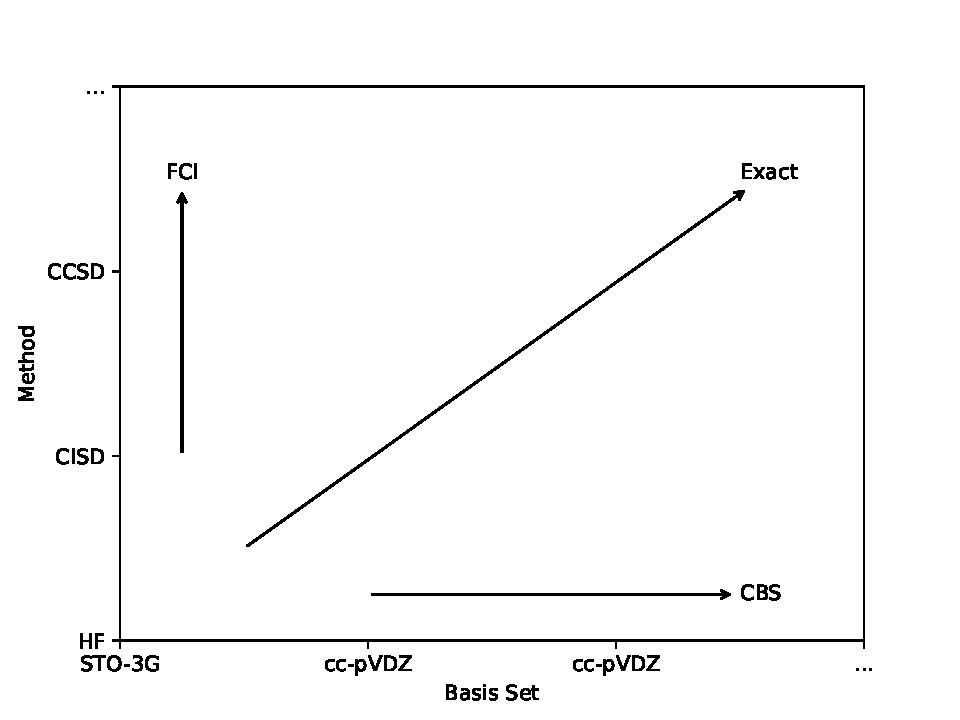
\includegraphics[width=0.8\textwidth]{figures/intro/hierarchies.pdf}
    \caption{A sketch for the hierarchy of theories and basis sets. There are two axes on which to systematically improve until reaching the exact solution to the time-independent Schr\"odinger equation under the \gls{BOA}: increasing basis set size (x axis) and increasing the level of theory (y axis). For most of this dissertation, we assume to be at or close to the highest level of theory (the FCI limit), as we mostly employ \gls{FCIQMC}. We therefore focus on methods of rapidly converging to the \gls{CBS} limit without the inherently expensive process of adding more basis functions.}
    \label{fig:hierarchies}
\end{figure}

% For so-called ``weakly-correlated'' electron systems, the \gls{HF} method or a modest improvement thereof is sufficient. However, for ``strongly-correlated'' electron systems, the \gls{HF} method can fail completely, not even describing the system qualitatively correctly.


\subsection{Configuration Interaction}
\label{sec:ci}

\Gls{CI} is perhaps the most conceptually straightforward post-Hartree-Fock method. Instead of using a single \gls{SD}, we approximate the wave function as a linear combination of \glspl{SD}. That is,
\begin{equation}
\ket{\Phi_\mathrm{CI}} = \sum_p c_p\ket{D_p}
\end{equation}
where $\ket{D_p}$ is a \gls{SD}. This may alternatively be written\footnote{We adopt the common notation convention where $i,j,k,...$ denote occupied orbitals, $a,b,c,...$ virtual (or unoccupied) orbitals, and $p,q,r, ...$ unspecified.}
\begin{equation}
\label{eq:ci}
\ket{\Phi_\mathrm{CI}} = (\one + \sum_{ia}c_i^a\hat a_a^\dag\hat a_i +
\sum_{ijab}c_{ij}^{ab} a_a^\dag a_b^\dag a_i a_j+...)\ket{\Phi_0}
\end{equation}
where the number of terms in the sum depends on how many excitations we consider, i.e. how far we truncate the \gls{CI} expansion. The energy and wave function are then found as the lowest eigenvalue and corresponding eigenvector, respectively, of the Hamiltonian written in the basis of these \glspl{SD}. This can be done, for example, by exact diagonalisation. If all possible excitations are considered, then we have reached the \gls{CBS} limit, and the solution is exact within that basis set.

\begin{figure}[htbp]
    \centering
    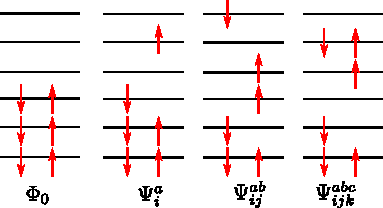
\includegraphics{figures/intro/configurations.pdf}
    \caption{Illustration of a \gls{RHF} reference and examples of single-, double-, and triple-excitations. The method CISDT, for example, would consider all determinants of the forms illustrated.}
    \label{fig:excitations}
\end{figure}

There are some important limitations to this method, however. Perhaps most notable is that the \gls{CI} method is not size consistent. For two noninteracting systems $A$ and $B$, we expect the composite system $A+B$ to have energy equal to the sum of that for $A$ and $B$, i.e. $E_{A+B}=E_A+E_B$. However, within a truncated \gls{CI} method, this is not the case\footnote{Of course, in \gls{FCI} we necessarily have size consistency, since we have the exact solution for the basis set.}, due to the additive ansatz \ref{eq:ci}.

Additionally, if we wish to go to the \gls{FCI} limit and ensure size consistency and accurate results, we once again have bad scaling, as discussed in section \ref{sec:matrix}. However, there exist sparse diagonalisation routines that need not store the entire matrix $H$, such as the Davidson,\cite{davidsonIterative1975} Lanczos,\cite{lanczosIteration1950} and Arnoldi\cite{arnoldiPrinciple1951} (for non-Hermitian $H$) methods, which target the ground state and need to store only a fraction of the matrix. Still, these scale with the size of the eigenvector, which is still prohibitively expensive for large systems. A more practical approach to reaching \gls{FCI} accuracy will be discussed later in section \ref{sec:fciqmc}, where we discuss the \gls{FCIQMC} algorithm.

\subsection{Multi-Configurational Self-Consistent Field}

As a generalisation of the \gls{HF} method, \gls{MCSCF} is particularly well-suited for problems with static correlation.\cite{helgakerMolecular2014,eadeDirect1981,roosNew1972} As in \gls{HF}, we minimise the electronic energy with respect to variational parameters; however, now we also simultaneously minimise with respect to expansion coefficients for a set of configurations (e.g. \glspl{SD}). i.e. consider the MCSCF wave function
\begin{equation}
\ket{\kappa,\bm c} = e^{-\kappa}\sum_ic_i\ket{D_i},
\end{equation}
where $\kappa$ is familiar from HF, and the $c_i$ coefficients farmiliar from \gls{CI}. In MCSCF, we optimise
\begin{equation}
E_\mathrm{MCSCF} = \frac{\bra{\kappa,\bm c}H\ket{\kappa,\bm c}}{\bra{\kappa,\bm c}\ket{\kappa,\bm c}}.
\end{equation}

Like in HF, the variational parameters appear nonlinearly and must be optimised iteratively. Determining an appropriate set $\{\ket{D_i}\}$ tends to be challenging, and even for small systems generating an MCSCF wave function can prove intractible.

\subsubsection{Complete Active Space Self-Consistent Field}
One ``flavour'' of \gls{MCSCF} that has proven particularly successful is \gls{CASSCF}.\cite{olsenCASSCF2011,roosComplete1980,siegbahnComparison1980,siegbahnComplete1981} In CASSCF, instead of inspecting individual configurations, we consider a set of configurations that satisfy a set of criteria. In particular, we partition the orbitals into three sets: the core, active, and virtual (unoccupied) regions. The core orbitals, as alluded to in section \ref{sec:core_electrons}, are approximated to be doubly occupied. The virtual orbitals are approximated to always be unoccupied. The active orbitals are the remaining orbitals, which can have occupations between 0 and 2.

The MCSCF expansion is found by considering all possible excitations of the active electrons in the active space. Notice that in the limit of an empty active space, we recover the \gls{HF} method, and in the limit of an active space containing all orbitals, we recover the \gls{FCI} method.

% might want to include a graphic for CAS space partitioning (or not idk)

\subsection{Perturbation Theory}
\label{sec:perturbation-theory}

Perturbation theory is a set of approximate mathematical methods for solving problems involving small disturbances (perturbations) to a problem with a known solution (the unperturbed problem). If these perturbations are not too large, then the solution of the perturbed problem is close to that of the unperturbed problem, and can be expressed as the solution of the unperturbed problem plus some corrections. Perturbation theory fails, however, if the perturbation is large.

\subsubsection{Rayleigh-Schr\"odinger}

Perturbation theory applied to time-independent problems is sometimes referred to as Rayleigh-Schr\"odinger perturbation theory.\cite{sakuraiModern2017,rayleighTheory1945,schrodingerQuantisierung1926} Consider a Hamiltonian,
\begin{equation}
H_\mathrm{PT} = H_0 + \lambda H',
\end{equation}
where $H_0$, referred to as the unperturbed Hamiltonian, $\lambda$ is an arbitrary (real) parameter controlling the strength of the perturbation, and $H'$ is the perturbation. We assume that we know the exact solution to $H_0$, such that we have all eigenstates $\{\ket{\Psi_n^{(0)}}\}$ and their corresponding eigenvalues $\{E_n^{(0)} \}$.

To obtain the solution to the true Hamiltonian $H$, we expand in terms of the perturbation $\lambda$,
\begin{equation}
\ket{\Psi_n} = \sum_{k=0}^\infty \lambda^k\ket{\Psi_n^{(k)}}
\end{equation}
and
\begin{equation}
E_n = \sum_{k=0}^\infty \lambda^kE_n^{(k)}.
\end{equation}
Since in this work we are generally interested in the ground state, we are typically targeting $n=0$.

By inserting these expansions into the time-independent Schr\"odinger equation, we equate terms of the same order in $\lambda$, which leads to the corrections to the energy and wave function. We may then truncate the expansion to some order. This allows for a systematically improvable result.

\subsubsection{M{\o}ller-Plesset}

M{\o}ller-Plesset perturbation theory\cite{mollerNote1934} is a special case of Rayleigh-Schr\"odinger perturbation theory, and is the variant most commonly seen in quantum chemistry.

In M{\o}ller-Plesset perturbation theory, the unperturbed Hamiltonian is chosen to be the Fock operator \ref{eq:fock-operator}. The perturbed Hamiltonian is known as the fluctuation potential and is the difference between the true Coulomb interaction and the effective one-electron potential discussed in section \ref{sec:hf}.

That is,
\begin{equation}
    H_0 = f, \hspace{10pt} H' = \sum_{i<j} r_{ij}^{-1}-V_\mathrm{eff} = H-H_0.
\end{equation}
If we apply Rayleigh-Schr\"odinger perturbation theory, we find the zeroth order wave function to be the \gls{HF} wave function,
\begin{equation}
    \ket{\Psi_0^{(0)}} = \ket{\Phi_0}, \hspace{10pt}
    f\ket{\Phi_0} = \underbrace{\sum_i\epsilon_i}_{E_0^{(0)}}\ket{\Phi_0}
    % , \hspace{10pt} E^{(0)} = E_\mathrm{HF}.
\end{equation}
where we have also identified the zeroth-order energy as the sum of orbital energies $E^{(0)}=\sum_i\epsilon_i$. With a bit more busywork, we get
\begin{align}
    E^{(1)} &= \bra{\Psi_0^{(0)}}H'\ket{\Psi_0^{(0)}} = \bra{\Phi_0}H'\ket{\Phi_0} \\
    E^{(2)} &=
    \sum_{n>0} \frac{|\bra{\Psi_n^{(0)}}H'\ket{\Psi_0^{(0)}}|^2}{E_0^{(0)}-E_n^{(0)}} =
    -\sum_{i>j,a>b}\frac{|\bra{\Phi_{ij}^{ab}}H'\ket{\Phi_0}|^2}{\epsilon_a+\epsilon_b-\epsilon_i-\epsilon_j},
\end{align}
where $\ket{\Phi_{ij}^{ab}}=a_a^\dag a_b^\dag a_ia_j\ket{\Phi_0}$ is a doubly-excited state with respect to the HF wave function, and $\epsilon_a+\epsilon_b-\epsilon_i-\epsilon_j = E_0^{(0)} - E_n^{(0)}$ is the energy difference between two eigenstates of the Fock operator.

Some features worth noting about M{\o}ller-Plesset perturbation theory:
\begin{itemize}
    \item The sum of zeroth- and first-order energies is the HF energy: $E_\mathrm{HF} = E_0^{(0)} + E_0^{(1)}$.
    \item By the variational principle, $E_0^{(0)}<E_n^{(0)}$ for all $n>0$ (except for degenerate ground states), so $E_0^{(2)}<0$, i.e. the energy always decreases.
    \item If the ground state is degenerate, the term diverges. It might be possible to lift the degeneracy by a change of basis, however.
    \item If the \gls{HF} solution is already a good approximation for the system, then M{\o}ller-Plesset perturbation theory can provide surprisingly good (and size consistent) results. Hence, this method is typically only applicable to single-reference problems (i.e. those without strong static correlation).
\end{itemize}

While higher-order approaches exist and see use, the most popular is \gls{MP2}, due to its excellent compromise between cost and accuracy. That is, for only a little extra work after a successful \gls{HF}, applying \gls{MP2} can improve our results considerably.

\subsection{Coupled Cluster Theory}

The lack of size consistency in \gls{CI} theory arises from the linear ansatz in section \ref{sec:ci}. By instead using an exponential ansatz, we arrive at one of the most successful theories in electronic theory, \gls{CC}.\cite{cizekCorrelation1966,cizekCorrelation1971,paldusTimeIndependent1975,shavittManyBody2009} While the methods presented here are inherently single-reference and build on a single \gls{SD}, multi-reference generalisations to \gls{CC} theory exist and are the study of active research.\cite{aotoInternally2016,evangelistaPerspective2018,hanauerPilot2011,jankowskiApplicability1992,jeziorskiCoupledcluster1981,kohnImproved2020} Therefore, the presented ``flavours'' of \gls{CC} are generally expected to fail for systems with strong static correlation.

\subsubsection{Standard Coupled Cluster}

To ensure a multiplicatively-separable wave function, we use a multiplicative ansatz,
\begin{equation}
    \label{eq:cc-ansatz}
\ket{\Psi_\mathrm{CC}} = \e^T\ket{\Phi_0},
\end{equation}
where $\ket{\Phi_0}$ is the reference (typically \gls{HF}) wave function, and $T$ is the cluster operator. The cluster operator is defined $T = T_1 + T_2 + T_3 + \cdots$, where $T_n$ is the $n$-body cluster operator, made up of all possible $n$-body excitations, for example, $T_1 = \sum_{i,a}t_{ia}a_a^\dag a_i$ for the one-body cluster operator, and $T_2 = \sum_{i<j,a<b}t_{ij}^{ab}a_a^\dag a_b^\dag a_j a_i$ for the two-body cluster operator.

It is worth noting that \gls{CC} and \gls{CI} are identical, differing only in their parametrisation, when neither are truncated. They both provide \gls{FCI}-level accuracy.

By inserting equation \ref{eq:cc-ansatz} into the time-independent Schr\"odinger equation and pre-multiplying by $\e^{-T}$, we obtain

\begin{align}
    \bra{\Phi_0}\e^{-T} H \e^T\ket{\Phi_0} &= E \\
    \label{eq:cc-schrodinger}
    \bra{\Phi_{ij...}^{ab...}}\e^{-T} H \e^T\ket{\Phi_0} &= 0
\end{align}
where $\ket{\Phi_{ij...}^{ab...}}$ is a $n$-body excitation with respect to the reference wave function.

Note, however, that these equations do not rely on the Variational Principle. Instead of minimising a functional, we solve equations \ref{eq:cc-schrodinger} for the amplitudes, which give the energy. While we still cannot reasonably always include all excitations in the cluster operator $T$, due to the multiplicative ansatz, even if we truncate the cluster operator, we get size-consistent results. In particular, any truncated CC wave function ansatz will contain contributions from all determinants in Fock space. The simplest CC truncation commonly used is the \gls{CCSD} method. In a sense, \gls{CCSD} and any other truncated CC method is an approximation for \gls{FCI} where the coefficients are not approximated to be zero (like in \gls{CI}) but instead the higher-order excitations terms are generated from the lower-order excitation terms in a size-consistent fashion.

CC theory owes much of its success to its high accuracy at a reasonable cost. \gls{CCSD} and \gls{CCSDT} in particular scale as $\mathcal{O}(M^6)$ and $\mathcal{O}(M^8)$ respectively, with $M$ the number of spatial orbitals. Every additional set of excitations incurs an additional factor of $\mathcal{O}(M^2)$ scaling.

\subsubsection{Distinguishable Cluster Theory}

The more recently-developed \gls{DCSD} method's central philosophy is removing irrelevant or nonphysical terms while maintaining many of CC's desireable properties, such as size consistency.\cite{katsCommunication2013}

This method was shown to give quantitatively better results than standard CC for a variety of systems, and qualitatively correct results for systems where CC can fail spectacularly, such as the N$_2$ binding curve. Since its first publication, \gls{DC} has been extended to explicitly-correlated F12 theory,\cite{katsAccurate2015} \gls{EOM},\cite{rishiExcited2017} tailored coupled cluster,\cite{vitaleFCIQMCTailored2020} and more.

\subsubsection{Combining Coupled Cluster with Perturbation Theory}

It is possible to avoid the computationally-expensive scaling of CC somewhat, by treating some terms perturbatively. The most famous of these is the \gls{CCSD(T)} method,\cite{raghavachariFifthorder1989} in which the single- and double-excitations are treated fully, whereas the triple-excitations are treated as perturbations, as in section \ref{sec:perturbation-theory}.

\gls{CCSD(T)} scales as $\mathcal{O}(M^7)$ and for the price provides extremely accurate results. The perturbative correction is a step that is applied only once at the end of a \gls{CCSD} calculation. This is why sometimes this method is referred to as the ``gold standard'' of quantum chemistry.

% \subsection{Density Matrix Renormalisation Group}

% ch 1
% introduction and context
% The quantum many-body problem, the TISE, in principle have everything but it's exceedingly difficult in practice, strong vs weak correlation, need for interesting materials and even small molecules to understand e.g. Haber-Bosch process and nitrogen fixation, mention multiscale methods (see Mona's notes?)
% scope of the thesis
% electronic structure theory
% Hartree-Fock Theory
% post-HF methods


% ch 2
\chapter{Explicitly Correlated Methods}
\label{chap:explicit}

With the advent of modern computers combined with a vast array of sophisticated algorithms from which to choose, \emph{ab initio} quantum chemistry has become a tremendously powerful tool, going beyond the study of small atoms, to molecules and solids, and are among the most effective and systematically improvable techniques to date. Nevertheless, convergence to the \gls{CBS} limit is notoriously slow.

In particular, consider the popular basis set family developed by Dunning and coworkers, \gls{cc-pV$X$Z}.\cite{dunningGaussian1989a,woonGaussian1993,woonGaussian1994,petersonBenchmark1994,wilsonGaussian1996}
The size of these basis sets scale as $M\in\mathcal{O}(X^3)$, and since for standard post-Hartree-Fock discussed in chapter \ref{sec:post-hf} we require four-index integrals, our computation time will scale at least as $t\in\mathcal{O}(X^{12})$.\cite{klopperR122007}

Meanwhile, the \gls{CBS} correlation error scales as $\epsilon\in\mathcal{O}(X^{-3})$ \cite{helgakerBasisset1997,halkierBasisset1998} or $\epsilon\in\mathcal{O}(M^{-1})$,\cite{klopperInitio1995} resulting in $t\in\mathcal{O}(M^{-\frac 14})$. Thus, the methods discussed so far come with the painful cost of requiring very large basis sets to approach high-accuracy results.

Explicitly correlated methods are a class of electronic structure methods specifically designed to address this unfavourable scaling by explicitly including the interelectronic distance $r_{12}$, and is the subject of this chapter. As the R12/F12 family of methods is the most mature of the explicitly correlated electronic structure methods, many reviews focusing on this topic already exist. This chapter in particular is in large part based on three reviews: references \citenum{klopperR122007}, \citenum{gruneisPerspective2017} and \citenum{hattigExplicitly2012}.


\section{The Cusp Conditions}
\label{sec:cusp}

Consider two charged point particles in a system described by the Hamiltonian of equation \eqref{eq:elec_hamiltonian_2q}. By the Schr\"odinger equation, the local energy
\begin{equation}
    E_L\mathdef \frac{H\Psi}{\Psi}
\end{equation}
must be constant in the exact solution. However, when these two particles coalesce, i.e. $r_{12}\to 0$, the Coulomb potential, $r^{-1}$, diverges. Thus, for the local energy to be constant, we must have that near coalescence points, the kinetic energy exactly cancels the Coulomb energy. A more formal treatment of this argument leads to the electron-electron Kato cusp condition,\cite{katoEigenfunctionsManyparticleSystems1957a}
\begin{equation}
    \label{eq:cusp}
    \left.\widetilde{\frac{\partial \Psi}{\partial r_{12}}}\right|_{r_{12}\to 0}
    = \frac 12 \Psi(r_{12}=0)
\end{equation}
where the tilde represents spherical averaging.

This cusp condition was also later generalised.\cite{packCuspConditionsMolecular1966,kurokawaChapterTwoGeneral2016}
Early literature on the subject suggested that the success of explicitly correlated methods were due to the superior description of short-range correlation effects, and in particular in their much more faithful capturing of the cusp conditions like equation \ref{sec:cusp}.\cite{roothaanAnalytical1960,watsonApproximate1960,weissConfiguration1961,schwartzGround1962}
However, further study found that the correlation error from a bad description of the wave function around a small sphere centred on the cusp is actually negligible.\cite{coulsonElectron1961,gilbertInterpretation1963,prendergastImpact2001,klopperR122007} Instead, the success of explicitly correlated methods is actually due to the superior description of the overall shape and size of the Coulomb hole, which has a radius on the order of the atomic radius.

To understand why gaussian-type basis sets fail so spectacularly at capturing the cusp behaviour, it is instructive to consider a simpler example, like that of approximating $|x|$ by its Fourier decomposition. Such an illustration is found in figure \ref{fig:cusp}. It is also worth noting that \glspl{STO} do not suffer as badly from this limitation,\cite{kongExplicitly2012} but as discussed in chapter \ref{sec:orbitals}, they are unsuccessful due to their lack of practicality.

% \todo{would be nice to think of other ways to add images}

\begin{figure}[htbp]
    \centering
    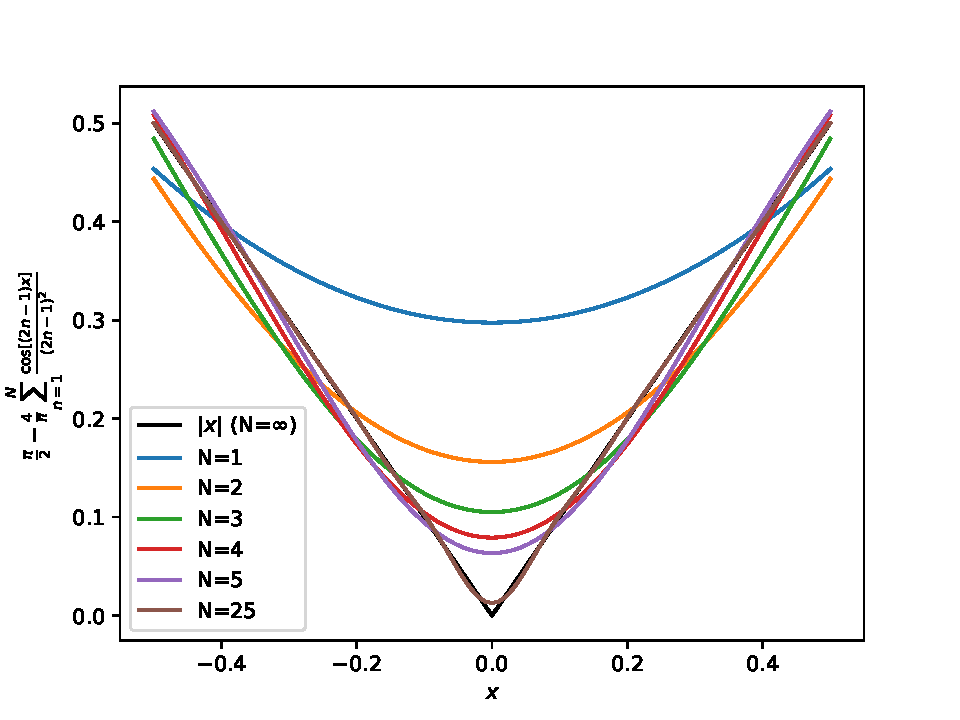
\includegraphics{figures/explicit/cusp.pdf}
    \caption{A toy example of the Coulomb cusp. Here, the Fourier expansion $x\approx\frac{\pi}{2} - \frac {4}{\pi} \sum_{n=1}^N\frac{\cos[(2n-1)x]}{(2n-1)^2}$ is plotted for a few values of $N$, including the exact solution. As can be seen, even for many terms, the Fourier expansion is a poor descripter in the cusp region. Indeed, the only way to describe it exactly is with an infinite number of terms.}
    \label{fig:cusp}
\end{figure}

\section{Hylleraas Methods}

Almost 30 years prior to Kato's landmark paper describing cusps in the analytical form for the wave function, there was already work being done to understand the significance of including $r_{12}$ terms in the wave function. Instead of being motivated by rigorous mathematics like Kato's, Slater was motivated by studies in the He atom. In particular, he tried to construct a wave function which faithfully represents both the core region as well as the Rydberg limit (i.e. a highly excited atom where the electron is very far from the nucleus).\cite{kongExplicitly2012,grynbergIntroduction2010,slaterCentral1928,slaterNormal1928} This led him to suggest multiplying the wave function by a factor
\begin{equation}
    \e^{-2(r_1+r_2)+r_{12}/2},
\end{equation}
which can easily be shown to satisfy the cusp equation \eqref{eq:cusp}.

However, the first successful explicitly correlated electronic structure calculation is typically attributed to Hylleraas,\cite{hattigExplicitly2012} where he aimed to improve convergence of orbital expansions for helium.\cite{hylleraasUeber1928,hylleraasNeue1929} In this method, the coordinates $s\mathdef r_1+r_2$, $t\mathdef r_1 - r_2$ and $u\mathdef r_{12}$ are used to construct the wave function
\begin{equation}
    \Psi_N(s,t,u) = \e^{-\alpha s}\sum_{k}^N c_ks^{l_k}t^{2m_k}u^{n_k}.
\end{equation}

In particular, using only three terms ($N=3$), and variationally optimising for the parameters $c_1,c_2,c_3$, Hylleraas was able to reach within 1.3 millihartree from the exact result.

Since then, there was rapid development on this approach and combining it with \gls{CI} (which came to be known as the CI-Hyl methods).
\cite{largo-cabrerizoHylleraasCI1987,jamesGround1933,kolosAccurate1964,perkinsAtomic1968,perkinsAtomic1969,simsCombined1971,simsOneCenter1971,claryHylleraastype1977,claryCIHylleraas1976} In CI-Hyl methods, the wave function is expanded as in \gls{CI},
\begin{equation}
    \Psi = \sum_k c_k \Phi_k
\end{equation}
where
\begin{equation}
    \Phi_k = \mathcal{A} r^{\nu_k}_{ij}\prod_i\chi_{k_i}(\bm x_i)
\end{equation}
where ${\chi_k}$ is a spin-orbital basis and $\mathcal{A}$ is the antisymmetriser operator.

However, CI-Hyl methods were to eventually fall out of favour. This is because the expansions involve exceedingly difficult integrals involving many electrons and over products of correlation factors. This significantly restricts the tractibility and scalability of the method, and it has since largely gone unused.

\section{Explicitly Correlated Gaussians}

Boys\cite{boysIntegral1960} and Singer\cite{singerUse1960} independently introduced gaussian basis functions with explicit correlation for calculations on molecules.\cite{mitroyTheory2013} These methods are referred to as \glspl{ECG}, or in the case of functions of two electrons, \glspl{GTG}. A spherical \gls{GTG} may be written (with nuclar coordinates $\bm R_1$ and $\bm R_2$) as
\begin{equation}
    g(\bm r_1, \bm r_2) = \exp(-\zeta_1|\bm r_1 - \bm R_1|^2 - \zeta_2|\bm r_2 - \bm R_2|^2 - \gamma|\bm r_1 - \bm r_2|^2).
\end{equation}
This can be interpreted as two $s$-type orbitals and an interelectronic correlation factor $\e^{-\gamma r_{12}}$.
While they do not have the correct cusp behaviour, much like how gaussian basis functions approximately capture the electron-nuclear cusp, a linear combination of \glspl{GTG} approximatelycapture the electron-electron cusp.

One major strength of this approach is that all integrals have closed-form algebraic expressions,\cite{lesterGaussian1964} and avoids nonlinear optimisation.\cite{bukowskiNew1994,perssonAccurate1996} \Gls{ECG} methods have been extended to post-Hartre-Fock methods, such as MP2\cite{panGaussian1970,panElectron1972}, and methods to avoid its many difficult integrals have also been developed.\cite{szalewiczNew1982,szalewiczAtomic1983,wenzelAtomic1986,szalewiczAtomic1984,tewWeak2007}

While not as popular as F12 methods (see section \ref{sec:f12}), \glspl{ECG} have been used for highly accurate variational calculations,\cite{korobovCoulomb2000} as well as for applications outside of standard electron structure theory, such as bosons,\cite{vargaPrecise1995} positronium (a bound state of an electron and a positron),\cite{bubinGroundstate2011} and non-Born-Oppenheimer systems.\cite{stankeNonBornOppenheimer2009}

\section{F12 Methods}
\label{sec:f12}

The most influential explicitly correlated class of methods to date are the F12 methods. The core principle of these methods is to augment the wave function from a conventional (typically \gls{SD}) basis with an explicitly-correlated correction, called the F12 (or R12) correction. The original formulation\todo{cite Kutzelnigg} parametrised a two-electron system (such as helium) wave function as
\begin{equation}
    \ket\Psi = (1+tQ_{12}r_12)\ket{\Psi_0}+\sum_{p}t_{p}\ket{\Psi_{p}}
\end{equation}
where $\Psi_0$ is a reference wave function (such as \gls{HF}), $\ket{\Psi_{p}}$ are excited-state \glspl{SD}, $t,t_{p}$ are parameters (``amplitudes'') to be optimised, and
\begin{equation}
    Q_{12} \mathdef \sum_{\alpha\beta}\ket{\alpha\beta}\bra{\alpha\beta}
\end{equation}
is referred to as a ``strong orthogonality projector'', which ensures the $r_{12}$ term is orthogonal to the reference and singly-excited determinants. Here $\alpha,\beta$ refer to virtual orbitals in the formally complete basis. The fact that, due to $Q_{12}$, the $r_{12}$ term commutes with the standard excitation operators aids in including this explicit correlation into conventional electron correlation methods.

% I think for this section I will largely be pulling from section 4 of \supercite{shiozakiMultireference2013}

% \subsection{A Historial Perspective: R12 Methods}
\todo{... see review papers haettig pg 30 for basic intro then 35 - 50 then excited state papers}

\todo{revisit}
brief mention of how it builds on gaussian-type geminals

% \subsection{}

\todo{make sure to include some excited state information}

\todo{mention but maybe don't go into too much detail on MR-F12 methods}

\section{The Transcorrelated Method}
\label{sec:tc}
\todo{brief recap of Boys-Handy method, some extensions by other people, and how it is used in our group}

Hirschfelder first introduced a similarity transform method \cite{hirschfelderRemoval1963}

then was worked on by Boys and Handy \todo{cite}, to be discussed here

uses ideas from \gls{VMC}, discussed more in section \ref{sec:vmc}.

recent renewal of interest (lots and lots of citations) with various applications, including DMRG, quantum computing, etc.

will talk in more detail about the Jastrow factor in section \ref{sec:jastrow} since it is also used in vmc

\todo{also mention biorthogonal orbitals etc.}

\todo{short proof of isospectrality}

\todo{reference section \ref{sec:variational_principle} and how it is not trivial to make TC variational since the proof of the variational principle uses the Hermiticity of the operator}

\subsection{The Method of Boys and Handy}

\subsection{Modern Resurgence}
\todo{Also cite Werner and quantum computing people}


\subsection{Comparison to F12/R12}

discuss additive vs multiplicative ansatz

have some performance comparison plots, maybe can ask permission to reproduce from Evelin or someone else

also discuss many-body integrals for f12 vs at most 3-body for tc


\todo{Maybe have a picture of basis set convergence? Maybe even just HF, compare F12 vs TC vs Hyl(?) vs standard}

% explicit correlation
% R12/F12 theory
% transcorrelation


% ch 3
\chapter{Monte Carlo Methods}
\label{chap:qmc}
\todo{...}
\todo{look especially at thijssen and the foulkes review for these sections}

\gls{MC} methods are a class of numerical methods that use random sampling to numerically solve problems. It has found applications in an impressive range of fields, from physics to finance.\todo{citation} It is particularly useful for problems with high dimensionality, where deterministic methods are often impractical. In quantum chemistry and physics, since a `dimension' can refer to any degree of freedom, high-dimensional problems are commonplace, and so \gls{MC} methods are a natural choice.

While the name \gls{MC} was coined by Stanislav Ulam, after the famous casino in Monaco,\todo{citation} the foundational concept was already developed in the 18th century by the French mathematician Georges-Louis Leclerc, Comte de Buffon. As one of the earliest example applications, in the Buffon needle problem, one can randomly toss needles onto a lined sheet of paper and determine $\pi$.\todo{citation}

\section{Classical Monte Carlo Methods}

We start our discussion with classical \gls{MC} methods. We consider the classical textbook problem of calculating the value of $\pi$, then we give it a more rigorous framework.

\subsection{A Very Bad Game of Darts}

\subsection{A More Mathematical Description}

\subsection{The Metropolis-Hastings Algorithm}

\section{Going Quantum: Variational Monte Carlo}
\todo{make sure to mention the Jastrow factor}

\section{Diffusion Monte Carlo}
\todo{main point here is just its similarity to FCIQMC}

\section{Auxiliary Field Quantum Monte Carlo}

\section{The Fermion Sign Problem}
\todo{make sure to mention the fixed node approximation here}

\section{QMC Meets Electronic Structure: the FCIQMC Algorithm}
\label{sec:fciqmc}

\subsection{The Sign Problem in FCIQMC}

\subsection{The Initiator Approximation}

\subsection{Reduced Density Matrix Sampling}

\subsection{Combining TC with Modern Electronic Structure}

% Monte Carlo Methods
% classical MC - games in Monaco/calculation of pi
% VMC, Jastrow factor
% DMC
% FCIQMC (link to DMC)
% the sign problem
% combining TC and FCIQMC

% ch 4
% aim to be here around page 60-80
\chapter{Optimising Jastrow Factors for the Transcorrelated Method}
  \label{chap:opt}

This chapter is based in large part on the following paper, and most of the following discussion can already be found there:\\
\fullcite{hauptOptimizing2023}

Images have been reused from this paper (with permission).

\section{Introduction}

In this chapter, we investigate the use of flexible Jastrow factors and a novel optimisation strategy for use in \gls{TC} as introduced in section \ref{sec:tc}. As a brief recapitulation, the TC method amounts to a similarity transformation of the Hamiltonian $\hat H$, $\htc = \e^{-J}\hat H\e^J$. However, as this is a non-unitary trasformation, methods used to solve $\htc$ are in general not variational, and hence we are not guaranteed to converge to the \gls{CBS} limit from above. It is therefore important to choose $J$ wisely, as otherwise the method may be highly non-variational, and we may suffer from poor error cancellation.

As an illustration of the method, we compute the all-electron atomisation energies for the challenging first-row molecules C$_2$, CN, N$_2$ and O$_2$ and find that \gls{TC}-\gls{FCIQMC} (that is, \gls{FCIQMC} performed on a transcorrelated Hamiltonian) yields chemically accurate results using only a \vtz basis, which requires a much larger \vxz{5} basis for non-TC.

\section{Computational Details}
We compute the ground-state energies of the all-electron C, N, and O atoms, as well as that for the C$_2$, CN, N$_2$ and O$_2$ molecules at their equilibrium geometries,\supercite{fellerSurvey2008,bytautasCorrelation2005,hardingHighaccuracy2008} listed in table
\ref{table:bond_lengths}.
TC- and non-TC-FCIQMC calculations used \gls{HF} orbitals (restricted open-shell in the case of open-shell systems) expanded in the standard \vxz{X} family of basis sets.\supercite{dunningGaussian1989a}


\begin{table}[htbp]
    \centering
      \caption{
      Electronic ground states and equilibrium bond lengths used for the
      molecules considered in this work, following reference \citenum{fellerSurvey2008}.
    }
    \label{table:bond_lengths}
    \begin{tabular}{ccc}
      System & State & $r_\mathrm{eq}$ (\AA) \\
    \hline \hline
      C$_2$ & ${}^1\Sigma_g^+$ & $1.2425$ \\
      CN    & ${}^2\Sigma^+$   & $1.1718$ \\
      N$_2$ & ${}^1\Sigma_g^+$ & $1.0977$ \\
      O$_2$ & ${}^3\Sigma_g^-$ & $1.2075$ \\
    \hline
    \end{tabular}
\end{table}

The quality of the energy differences is assessed using the atomisation energies of these molecules. In order to determine if our methodology yields chemically-accurate, i.e. within an error of $1$ kcal/mol $\approx 1.6$ mHa, we also keep each individual error to be well within this threshold. We expect a total bias in our resulting relative energies of not more than $0.5$ mHa.

For all our calculations, we generate our orbitals and integration grids using \pyscf,\supercite{sunPySCF2018} optimise the Jastrow factors using the \casino continuum \gls{QMC} package,\supercite{needsVariational2020}, compute TC matrix elements using the \tchint library, for which more details are presented in \autoref{chap:pytchint}, and perform (TC-)FCIQMC calculations using the \neci package.\supercite{gutherNECI2020} FCIQMC energies reported are the standard HF-projected energies.

(TC-)FCIQMC values presented here were produced using a walker-number extrapolation scheme presented in another dissertation.\supercite{hosseiniCombining2024}

\section{Jastrow Factor}

In continuum quantum Monte Carlo methods, the Jastrow factor for a molecule is typically expressed as the sum of electron-electron, electron-nucleus, and electron-electron-nucleus terms,\footnote{Of course, these are not all the possible terms. We may, for example, also choose to include electron-nucleus-nucleus terms.}
\begin{equation}
    \label{eq:jastrow}
    J = \sum_{i<j}^Nv(r_{ij}) + \sum_i^N\sum_I^{N_A}\chi(r_{iI}) + \sum_{i<j}^N\sum_I^{N_A}f(r_{ij}, r_{iI}, r_{jI}),
\end{equation}
where $N_A$ is the number of nuclei, $N$ the number of electrons, and each of $u$, $\chi$, and $f$ are expressed as natural power expansions.\supercite{drummondJastrow} That is,
\begin{equation}
    \label{eq:dtn-jastrow-ee}
    v(r_{ij})    = t(r_{ij},L_v)
                    \sum_{k} a_k r_{ij}^k ,
\end{equation}
\begin{equation}
    \label{eq:dtn-jastrow-en}
    \chi(r_{iI}) = t(r_{iI},L_\chi)
    \sum_{k} b_k r_{iI}^k ,
\end{equation}
\begin{equation}
    \label{eq:dtn-jastrow-een}
    f(r_{ij}, r_{i}, r_{j}) = t(r_{iI},L_f) t(r_{jI},L_f)
    \sum_{k,l,m} c_{klm}
    r_{ij}^k r_{iI}^l r_{jI}^m ,
\end{equation}
where $\{a_k\}$, $\{b_k\}$, and $\{c_{klm}\}$ are linear parameters,
$L_v$, $L_\chi$, and $L_f$ are cut-off lengths, $t(r,L) = (1-r/L)^3
\Theta(r-L)$ is a cut-off function, and $\Theta(r-L)$ is the Heaviside
step function.

As described in chapter \ref{chap:explicit}, accurately describing the (electron-electron and electron-nucleus) Kato cusp conditions\supercite{katoEigenfunctionsManyparticleSystems1957a} substationally improves the accuracy of our method. Also, as described in chapter \ref{chap:qmc}, \gls{VMC} and \gls{DMC} methods sample electronic configurations $\{\bm R\}$ from a probability distribution based on an analytical trial wave function $\tilde\Psi_{\mathrm T}(\bm R)$ to produce a variational estimate of the total energy as an average of the local energy, $E_{\mathrm L}({\bm R}) = \tilde\Psi_{\mathrm T}^{-1}({\bm R}) \hat H({\bm R}) \tilde\Psi_{\mathrm T}({\bm R})$ over the sampled configurations. In the case of \gls{VMC}, accurate description of the electron-electron and electron-nucleus Kato cusp conditions suppresses extreme outliers in the local energy sampling, allowing meaningful wave function parameters.

The most obvious way to enforce the electron-electron and electron-nucleus cusp conditions is by enforcing them in the form of the Jastrow factor through the relevant terms, namely $v$ (equation \ref{eq:dtn-jastrow-ee}) for the electron-electron cusp, and $\chi$ (equation \ref{eq:dtn-jastrow-en}) for the electron-nucleus cusp. However, in the context of continuum \gls{QMC}, it has been found to be better\supercite{drummondJastrow,needsVariational2020,maScheme2005} to enforce the electron-nucleus cusp by modifying the $l=0$ ($s$-type) component of the cuspless molecular orbitals, $\phi(r)$, such that they exhibit a cusp.

Since we are interested in performing a post-Hartree-Fock calculation on $\htc$, such as \gls{FCIQMC}, it is preferable to use unmodified molecular orbitals from standard basis sets during the optimisation process. If we optimise the Jastrow factor in \gls{VMC} in the presence of cusp-corrected orbitals and then use them in TC-FCIQMC without the cusp-corrected orbitals, the Jastrow factor would be sub-optimal for the Hamiltonian, by construction.

Instead, we recast the cusp-correction scheme of \onlinecite{maScheme2005} as an electron-nucleus Jastrow factor term, called $\Lambda$, to be added (rather than replacing) the $\chi$ term of equation \ref{eq:dtn-jastrow-en}. We construct this term as

\begin{equation}
    \label{eq:cusp-corr-1}
    \Lambda(r)  = \left[ \ln \tilde \phi(r) - \ln \phi(r) \right]\Theta(r-r_{c}),
\end{equation}
where, adopting the notation of \onlinecite{maScheme2005}, $r_c$ is a cutoff radius, $\phi(r)$ is the $s$-type component of the target orbital, and $\tilde \phi(r)$ is its cusp-corrected counterpart,
\begin{equation}
    \label{eq:cusp-corr-2}
  \tilde \phi(r) = \e^{\sum_{l=0}^4 \alpha_l r^l} + C \quad,\quad r<r_{c}.
\end{equation}

Here, $\{\alpha_l\}$ are parameters determining the shape of the
corrected orbital and the shift $C$ is only set to a non-zero value in
the presence of nodes of $\phi(r)$ near the nucleus. More precisely, the shift $C$ is chosen such that $\tilde\phi(r_c)-C$ is of one sign within the radius $r_c$. This is necessary since we wish to impose an exponential correction, which is necessarily of one sign.

Following \onlinecite{maScheme2005}, we impose the cusp condition at $r=r_c$, as well as twice continuous differentiability at $r=r_c$. This leaves only $\alpha_0$ and $r_c$ as free parameters from equations \ref{eq:cusp-corr-1} and \ref{eq:cusp-corr-2}. $r_c$ is chosen to be small but within the same sign, as described above, while $\alpha_0$ is determined by enforcing smoothness for the so-call ``effective one-electron local energy'',
\begin{equation}
    E_L^s(r) \mathdef \tilde\phi(r)^{-1}\left[-\frac 12\nabla^2-\frac{Z_{\mathrm{eff}}}r\right]\tilde\phi(r).
\end{equation}
Here, the effective nuclear charge $Z_\mathrm{eff}$,
\begin{equation}
    Z_\mathrm{eff} = Z\left(1 + \frac{\eta(0)}{\tilde\phi(0)}\right)
\end{equation}
ensures that $E_L^s$ is finite at the origin, and is derived from the cusp condition. $\eta$ is the rest of the orbital, leftover from removing the $s$-type component.

Figure \ref{fig:cusp-term} illustrates the effect of using a $\Lambda$
term in practice.

\begin{figure}[htbp]
    \centering
    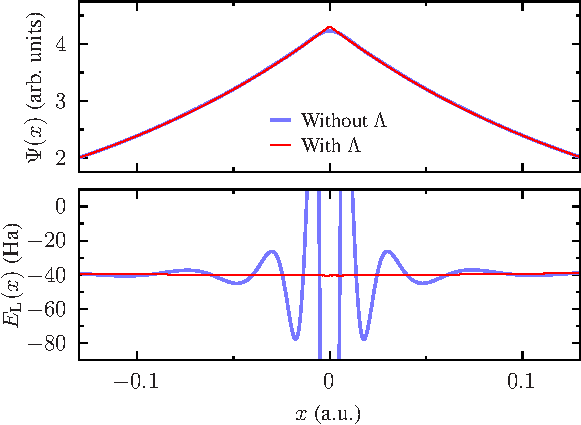
\includegraphics[width=0.8\columnwidth]{figures/optimisation/Fig/cusp-term-eps-converted-to}
    \caption{\gls{HF} wave function value and local energy as a function of the $x$ coordinate of an electron in a carbon atom as it crosses the nucleus at $x=0$, both with and without the $\Lambda$ cusp-correcting Jastrow factor term. This is in the \vdz basis.}
    \label{fig:cusp-term}
\end{figure}

For the calculations in this chapter, we use a total of $44$ optimisable Jastrow factor parameters for the atoms and homonuclear dimers, and $88$ parameters for CN. We keep the $L_v$, $L_\chi$ and $L_f$ cutoff lengths fixed at $4.5$, $4$, and $4$, for simplicity.

\section{Optimisation Strategy}

We optimise $J$ using \gls{VMC}. VMC provides a variational framework in which parameters $\bm \alpha$ present in a trial wave function $\Psi_\mathrm{T}$ can be optimised. In this chapter, $\ket{\Psi_\mathrm{T}} = \e^{J(\bm\alpha)}\ket{D_\mathrm{HF}}$.

Wave function optimisation is usually carried out using a correlated-sampling approach in which a set of $n_mathrm{opt}$ electronic real-space configurations ${\{\bm R}_{i}\}_{i=1}^{n_\mathrm{opt}}$ distributed according to the initial wave function squared, $|\Psi_\mathrm{T}({\bm R}; {\bm \alpha}_0)|^2$ is generated, and then a target function is minimised by varying $\bm\alpha$ at fixed ${\{\bm R}_{i}\}$.

The variational energy estimate for this trial wave function may be written
\begin{equation}
    E_\mathrm{VMC} = \frac{\bra{\Psi_\mathrm{T}} \hat H \ket{\Psi_\mathrm{T}} }{ \braket{\Psi_\mathrm{T}}{\Psi_\mathrm{T}} },
\end{equation}
which may be used as a target function, as presented in section \ref{sec:vmc}.

Another popular target function is the ``variance of the VMC energy,''\supercite{umrigarOptimized1988,kentMonte1999}
\begin{equation}
\sigma_\mathrm{VMC}^2 = \frac{\bra{\Psi_\mathrm{T}}(\hat H - E_\mathrm{VMC})^2\ket{\Psi_\mathrm{T}}}{\braket{\Psi_\mathrm{T}}},
\end{equation}
which reaches its minimum of zero when the trial wave function is an eigenstate of the Hamiltonian. In practice, minimising $\sigma_\mathrm{VMC}^2$ yields variational energies, but is affected by large fluctuations, as shown in this chapter.

In continuum QMC methods, modifications have been devised to
circumvent this problem, such as weight limiting, unreweighted
variance minimization, or the minimization of other measures of spread
such as the median absolute deviation from the median energy.\supercite{needsVariational2020}

The computational cost of optimizing Jastrow factors within VMC scales
as a small power of system size, typically estimated to be ${\mathcal
O}(N^3)$.

\subsection{Variance of the Reference Energy Minimisation}

In the context of TC, the reference energy
\begin{equation}
    E_\mathrm{ref} = \bra{D_\mathrm{HF}}\e^{-J}\hat H\e^J\ket{D_\mathrm{HF}}
\end{equation}
is of particular significance since it represents the starting point of a TC-FCIQMC calculation (i.e. the walker distributions at imaginary time $\tau=0$ has this energy). It is also the zeroth-order contribution to the TC-\gls{CC} energy.

We refer to its associated variance,
\begin{equation}
  \label{eq:var_eref_1}
  \sigma_\mathrm{ref}^2 =
    \bra{D_\mathrm{HF}}\e^{-J} (\hat H^\dag-E_\mathrm{ref})(\hat H-E_\mathrm{ref}) \e^J\ket{D_\mathrm{HF}}
\end{equation}
as the ``variance of the reference energy,'' which is easily evaluated for a finite VMC sample of size $n_\mathrm{opt}$ as the sample variance of the Slater-Jastrow energy over the HF distribution,
\begin{equation}
    S_\mathrm{ref}^2 =
      \frac 1 {n_\mathrm{opt}-1}
      \sum_{n=1}^{n_\mathrm{opt}}
        \left| \frac {\hat H({\bm R}_n) \Psi_\mathrm{SJ}({\bm R}_n)}
                     {\Psi_\mathrm{SJ}({\bm R}_n)} - {\bar E}_\mathrm{ref}
        \right|^2,
\end{equation}
% TODO : you will want to practice proving this, just in case for your defence
which tends to $\sigma_\mathrm{ref}^2$ as $n_\mathrm{opt}\to\infty$, where $\Psi_\mathrm{SJ}\mathdef \e^JD_\mathrm{HF}$ is the Slater-Jastrow wave function, $\{{\bm R}_n\}_{n=1}^{n_\mathrm{opt}}$ are electronic
configurations distributed according to $D_\mathrm{HF}^2$, and the VMC
estimate of the reference energy is
\begin{equation}
    {\bar E}_\mathrm{ref} =
      \frac 1 {n_\mathrm{opt}}
      \sum_{n=1}^{n_\mathrm{opt}}
        \frac {\hat H({\bm R}_n) \Psi_\mathrm{SJ}({\bm R}_n)}
              {\Psi_\mathrm{SJ}({\bm R}_n)}.
\end{equation}

% TODO: you will want to familiarise yourself with these papers
The variance of the reference energy has been used as a target function for optimising Jastrow factors for the TC method before, albeit in different theoretical frameworks.\supercite{handyMinimization1971,umezawaTranscorrelated2003}

To understand the physical significance of the variance of the reference energy, note that equation \ref{eq:var_eref_1} may be rewritten as
\begin{equation}
    \label{eq:varref-connectivity}
    \sigma_\mathrm{ref}^2 = \sum_{I\neq \mathrm{HF}}\bra{D_I}\htc\ket{D_\mathrm{HF}},
\end{equation}
where $I$ runs over a complete basis set.\footnote{Here we have a complete basis set because we are optimising with continuum Monte Carlo. If we were to optimise this by directly calculating the matrix elements in equation \ref{eq:varref-connectivity}, then the sum must be truncated. This is the subject of ongoing work.}

As evident by equation \ref{eq:varref-connectivity}, minimising $\sigma_\mathrm{ref}^2$ essentially amounts to minimising the coupling of the reference determinant with the remainder of the space, which in the context of FCIQMC translates to a reduced spawning rate from the reference determinant to its connected excited-state determinants, thereby increasing the amplitude of the reference determinant in the resulting CI vector.

Note also that if the Slater-Jastrow wave function were an exact eigenstate of $\hat H$, then a TC-FCIQMC simulation starting from the HF determinant would immediately converge to a strictly single-determinant solution. Although this ideal scenario cannot be achieved in practice, it nevertheless illustrates the potential benefits of obtaining a relatively single-reference CI solution by minimising this target function. We expect that this increased single-reference character will also benefit other approaches, particularly those based on single references, such as TC-CC.

We therefore investigate the performance of minimising the variance of the reference as an alternative to minimising the variance of the VMC energy. In figure \ref{fig:varmin-E-Eref}, we compare the VMC energy and variance obtained by variance minimisation methods along with energy-minimised\supercite{nightingaleOptimization2001,toulouseOptimization2007,umrigarAlleviation2007} results for reference, for the systems considerd in this chapter, using $n_\mathrm{opt}=10^5$ VMC configurations.

\begin{figure}[htbp]
    \centering
    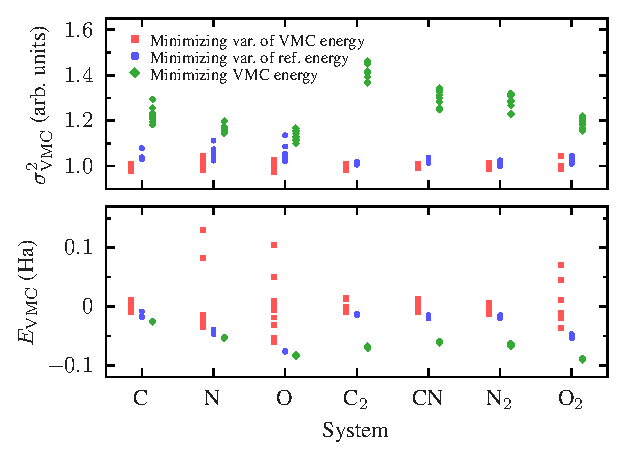
\includegraphics[width=0.8\textwidth]{figures/optimisation/Fig/varmin-E-Eref}
    \caption{Variance of the VMC energy (top) and VMC energy (bottom) of the systems considered in this chapter using the \vtz basis and Jastrow factors obtained by minimising the variance of the VMC energy (red squares), the variance of the reference energy (blue circles), or the VMC energy (green diamonds) in each of ten independent optimisation runs with $n_\mathrm{opt}=10^5$ VMC configurations. To ease comparisons, variances have been rescaled and energies shifted by their average values from minimising the variance of the VMC energy (i.e. the red squares average to a variance of $1$ and an energy of $0$ in the plot). The subpar ability of VMC energy variance minimisation to yield consistent VMC energies is evident in the bottom panel, suggesting to use the variance of the reference.}
    \label{fig:varmin-E-Eref}
\end{figure}
%
Minimizing the variance of the VMC energy produces lower average
values of $\sigma_\mathrm{VMC}^2$, as one would expect, but also erratic
VMC energies with very large standard deviations (up to $\sim50$ mHa
in our tests).
%
Minimizing the variance of the reference energy, on the other hand,
produces values of $\sigma_\mathrm{VMC}^2$ which are only slightly higher
on average than those obtained from minimizing the variance of the VMC
energy ($1$--$5\%$ in our tests), while producing more stable VMC
energies with much smaller standard deviations (up to $\sim3$ mHa in
our tests).
%
We therefore do not use ``regular'' variance minimization since it
introduces large stochastic noise, making it unsuitable for optimizing
Jastrow factors, and from this point on we use the term ``variance
minimization'' to refer to the minimization of the variance of the
reference energy.

\subsection{Choosing an Appropriate Sample Size}

While expectation values relevant for most continuum QMC calculations converge using relatively few VMC configurations, it has also been known\supercite{spinkTrion2016} that in order to converge other quantities, far more configurations are needed. That is, $n_\mathrm{opt}$ is larger. In the spirit of \gls{MC}, we may estimate the convergence of the expectation value for some quantity by performing multiple optimisation runs with different random number seeds but otherwise the same inputs. This would give us a standard deviation.

The value we want to converge in this case is not the VMC energy, nor the reference energy, but instead the TC-FCI energy. In practice, we use the uncertainty of the VMC estimate of the reference energy $\bar E_\mathrm{ref}$ as a proxy for the standard deviation of the TC-FCIQMC energy. This is justified because:
\begin{itemize}
    \item The standard deviation of the TC-FCIQMC energy is not larger than the standard deviation of the reference energy, as illustrated in figure \ref{fig:spread_c2_cc-pvdz}. It is usually significantly smaller thanks to the ability of TC-FCIQMC to conpensate for the presence of a bias in $E_\mathrm{ref}$ via the correlation energy.
    \item The standard deviation of the reference energy is not larger than the statistical uncertainty of the VMC estimate of the reference energy obtained with $n_\mathrm{opt}$ configurations. It is usually significantly smaller due to the use of variance reduction techniques in QMC.
\end{itemize}

\begin{figure}[htbp]
    \centering
    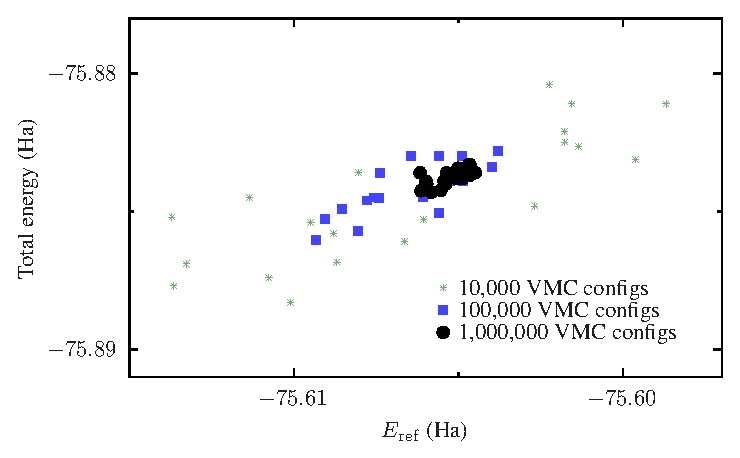
\includegraphics[width=0.8\textwidth]{figures/optimisation/Fig/spread_c2_cc-pvdz}
    \caption{TC-FCIQMC energy of the C$_2$ molecule using $10^6$ walkers with the \vdz basis as a function of the reference energy for multiple independent Jastrow factor parameter sets obtained by variance minimisation using three different VMC sample sizes. The horizonal spread is about $1.8$ times larger than the vertical spread, in line with the expectation that the standard deviation of the TC-FCIQMC energy is smaller than that of the reference energy.}
    \label{fig:spread_c2_cc-pvdz}
\end{figure}

For the atoms and molecules considered in this chapter, we use $n_\mathrm{opt}=2\times 10^7$ to yield TC-FCIQMC energies with standard deviations of less than $0.1$ mHa.

\subsection{Energy Minimisation}

The obvious alternative to variance minimisation is minimising the VMC energy,\supercite{nightingaleOptimization2001,toulouseOptimization2007,umrigarAlleviation2007} which, as already demonstrated in figure \ref{fig:varmin-E-Eref}, results in lower VMC energies but higher VMC variances.
Energy minimisation yields wave functions which minimise the statistical fluctuations of the local energy in DMC calculations\supercite{ceperleyStatistical1986} and is the typical choice for continuum QMC. However, for our purposes, it is unclear whether the resulting wave functions provide a better description of the system than those produced by variance minimisation.

In figure \ref{fig:bsdep-atoms-emin}, we compare the convergence with basis-set size of TC-FCIQMC total energies of the C, N, and O atoms using energy- and variance-minimised Jastrow factors. Variance minimisation appears to produce wave functions which converge quickly and largely variationally to the basis set limit, which energy-minimised wave functions tend to yield non-variational TC-FCIQMC energies which converge more slowly to the basis set limit.

\begin{figure}[htbp]
    \centering
    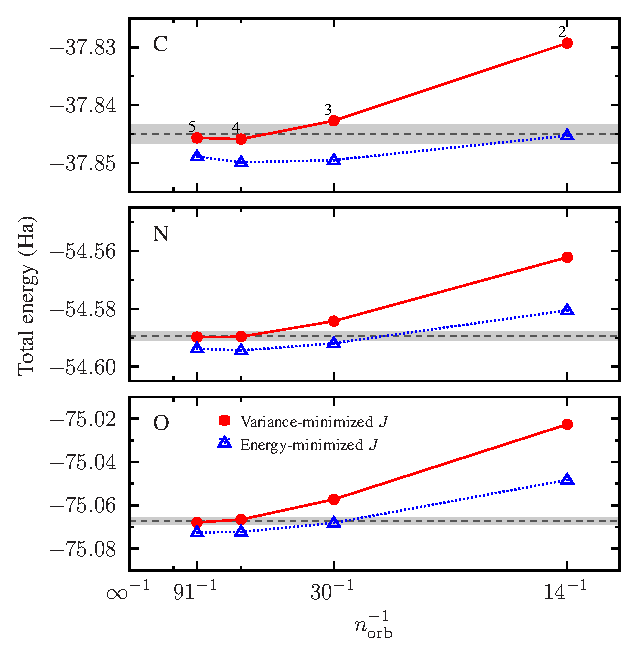
\includegraphics[width=0.8\textwidth]{figures/optimisation/Fig/bsdep-atoms-emin}
    \caption{Total energy of the C, N, and O atoms as a function of the reciprocal number of molecular orbitals in the \vxz{X} basis set family. The non-variational behaviour of up to about $5$ mHa is evident for the energy-minimised Jastrow factors, for which convergence to the exact energy as a function of basis-set size is slow. The shaded areas represent $\pm 1$ kcal/mol (so-call ``chemical accuracy'') around the exact non-relativistic total energy from reference \citenum{bytautasCorrelation2005}. Points in the top panel are annotated with the basis set cardinal number $X$.}
    \label{fig:bsdep-atoms-emin}
\end{figure}

In figure \ref{fig:bsdep-dimers-emin} we plot the atomisation energies of the dimers as a function of reciprocal basis-set size, again demonstrating variance-minimised Jastrow factors exhibit favourable convergence properties.

\begin{figure}[htbp]
    \centering
    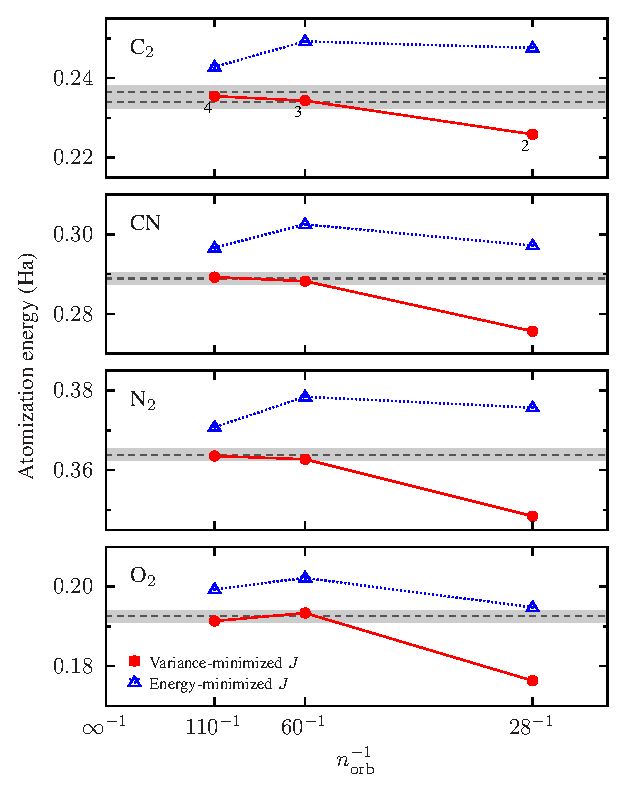
\includegraphics[width=0.8\textwidth]{figures/optimisation/Fig/bsdep-dimers-emin}
    \caption{Atomisation energy of the C$_2$, CN, N$_2$, and O$_2$ molecules as a function of the reciprocal of the number of molecular orbitals using the \vxz{X} family of basis sets and Jastrow factors obtained by variance and energy minimisation. The shaded areas represent $\pm 1$ kcal/mol around the theoretical estimate of the exact non-relativistic atomisation energies from references \parencite{fellerSurvey2008,bytautasCorrelation2005}}.
    \label{fig:bsdep-dimers-emin}
\end{figure}

Considering this evidence, we choose to use variance minimisation to optimise the Jastrow factors for subsequent post-HF calculations.

\section{Grid Sizes}

How matrix elements are evaluated is presented in \autoref{chap:pytchint}. As mentioned there, we use Treutler-Ahlrichs integration grids,
\supercite{beckeMulticenter1988,treutlerEfficient1995} which are atom-centred
grids constructed as the combination of a radial grid running up to
the Bragg radius and a Lebedev angular grid. These are obtained using \pyscf, which provides an integer parameter $l_\mathrm{grid}$ to control the grid density. Here we test grid errors by evaluating TC-FCIQMC energies at $l_\mathrm{grid}=1$--$5$ and defining the integration error as the difference of each of these results with the value obtained by linear extrapolation to the $1/n_\mathrm{grid}\to 0$ limit.

In figure \ref{fig:griderr-atoms} we plot the absolute integration error in the total energy of the atoms as a function of $1/n_\mathrm{grid}$ for \vdz, \vtz and \vqz basis sets. We find that the basis set size has little to no effect on the integration error.

\begin{figure}[htbp]
    \centering
    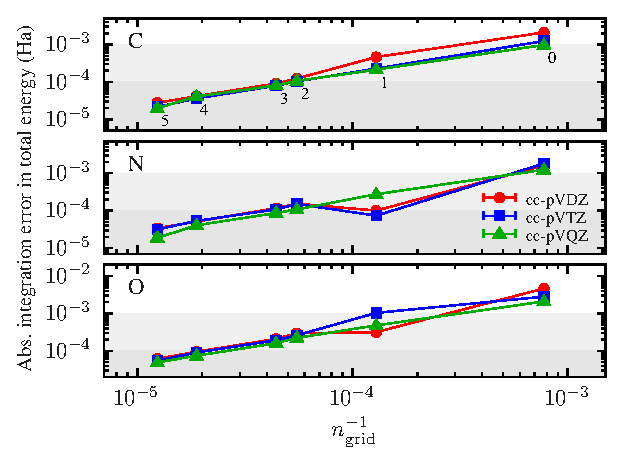
\includegraphics[width=0.8\textwidth]{figures/optimisation/Fig/griderr-atoms}
    \caption{Absolute integration errors in the total energy for the C, N, and O atoms as a function of the reciprocal of grid size using basis sets in the \vxz{X} family. The gray areas correspond to integration errors of less than $1$ and $0.1$ mHa. Points in the top panel are annotated with the value of \pyscf's grid density parameter.}
    \label{fig:griderr-atoms}
\end{figure}

In figure \ref{fig:griderr-dimers} we plot the absolute integration error in the total energies of the molecules, the atoms that conform them, and atomisation energies using the \vdz basis. We find integration-error cancellation in energy differences, with atomisation energy for all four molecules reaching $0.1$ mHa for $l_\mathrm{grid}=2$. This represents a $60$-point radial grid combined with a $302$-point angular grid, for a total of $18120$ grid points per atom. We use this throughout this dissertation.

\begin{figure}[htbp]
    \centering
    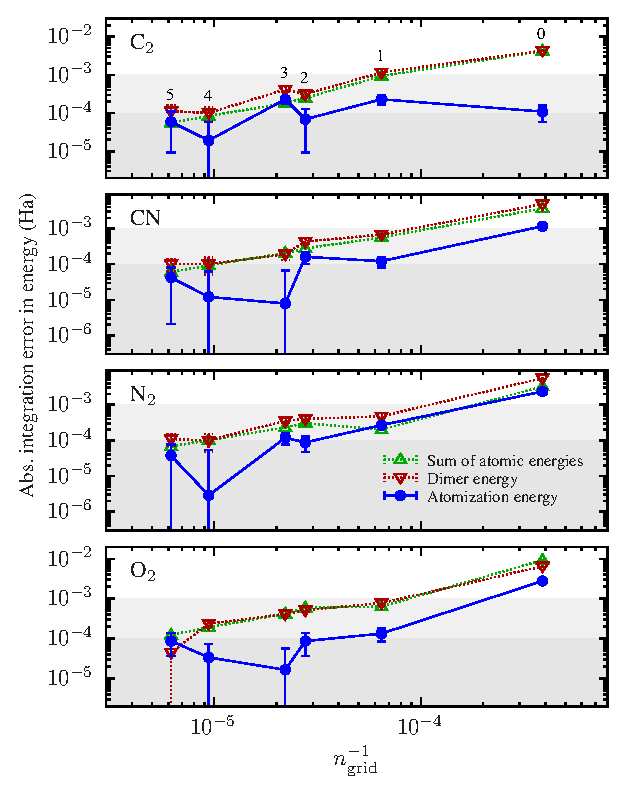
\includegraphics[width=0.8\textwidth]{figures/optimisation/Fig/griderr-dimers}
    \caption{Absolute integration error in the energy as a function of the reciprocal number of grid points used for the evaluation of TC integrals. The shaded areas correspond to integration errors of less than $1$ and $0.1$ mHa. Points in the top panel are annotated with the value of \pyscf's grid density parameter. These results demonstrate that $l_\mathrm{grid}=2$ is sufficient to achieve sub-mHa accuracy in total energies and sub-$0.1$-mHa accuracy in relative energies.}
    \label{fig:griderr-dimers}
\end{figure}


\section{Compactification of the CI Vector}
The more compact the CI wave function is, the easier it is for FCIQMC to sample the wave function accurately and the smaller the initiator error becomes. The TC method has already been shown to make CI wave functions more compact for the two-dimensional Hubbard model.\supercite{dobrautzCompact2019} Let $\{c_I\}$ be the $L^2$-normalized coefficients of the CI wave
function such that $\sum_I c_I^2=1$.
%
The quantity
%
\begin{equation}
  \label{eq:xi_compactness}
  \xi = \frac { c^\mathrm{(TC)}_\mathrm{HF} - c^\mathrm{(non-TC)}_\mathrm{HF} }{ 1 - c^\mathrm{(non-TC)}_\mathrm{HF} }
\end{equation}
%
is then a measure of the enhancement in the compactness of the wave
function, going from $0$ for no enhancement to $1$ if the TC wave
function becomes exactly single-determinantal.

From reference \citenum{dobrautzCompact2019}, TC yields a maximum of $\xi=0.64$ for the 18-site 2D Hubbard model. We find that the values of $\xi$ for atomic and molecular systems are not dissimilar from this, as shown in table \ref{table:l2_norms}.
%
\begin{table}[htbp]
    \centering
    \begin{tabular}{cccccccc}
            & C      & N      & O      &
              C$_2$  & CN     & N$_2$  & O$_2$  \\
    \hline \hline
    cc-pVDZ & $0.46$ & $0.63$ & $0.71$
            & $0.14$ & $0.23$ & $0.38$ & $0.53$ \\
    cc-pVTZ & $0.45$ & $0.61$ & $0.69$
            & $0.15$ & $0.24$ & $0.40$ & $0.55$ \\
    cc-pVQZ & $0.44$ & $0.60$ & $0.69$
            & $0.15$ & $0.24$ & $0.41$ & $0.57$ \\
    \hline
    \end{tabular}
    \caption{
      Enhancement of the compactness of the CI wave function, $\xi$ in
      Eq.\ \ref{eq:xi_compactness}, between our non-TC and TC-FCIQMC
      calculations.
    }
    \label{table:l2_norms}
  \end{table}

\section{Neglecting Three-Body Excitations}

As described in section \ref{sec:fciqmc}, sampling in FCIQMC involves spawning walkers from occupied determinants onto connected determinants. The $\hat L$ matrix, that is the three-body operator arising from the similarity transformation in TC, results in TC also connecting determinants by three-body excitations. This represents a huge increase in the connectivity of the Hilbert space compared to non-TC-FCIQMC.

These three-body excitations are represented by $L_{ijk}^{abc}$ where each index is distinct. These have been found to typically be small.\supercite{dobrautzPerformance2022} Moreoever, simultaneous interaction of three electrons is unlikely due to Pauli repulsion (as necessarily at least two of the electrons will be of the same spin). Therefore, we neglect these contributions. The only distinct six-index integrals that we must keep are those occupied in the HF determinant, as these matrix elements are necessary to evaluate the projected energy.

Neglecting pure three-body excitations reduces the amount of storage needed to hold $\hat L$ from $\mathcal{O}(M^6)$ to $\mathcal{O}(M^5+N^3M^3)$, where $M$ is the number of orbitals and $N$ is the number of electrons. Reduction factors obtains for the molecules studied in this chapter are reported in table \ref{table:no3_memory}.

\begin{table}[htbp]
    \centering
    \begin{tabular}{cccccccc}
            & C      & N      & O      &
              C$_2$  & CN     & N$_2$  & O$_2$  \\
    \hline \hline
    cc-pVDZ & $1.23$ & $1.17$ & $1.17$ &
              $1.87$ & $1.78$ & $1.78$ & $1.58$ \\
    cc-pVTZ & $2.04$ & $2.02$ & $1.93$ &
              $3.72$ & $3.66$ & $3.66$ & $3.46$ \\
    cc-pVQZ & $3.31$ & $3.44$ & $3.13$ &
              $6.60$ & $6.54$ & $6.57$ & $6.41$ \\
    \hline
    \end{tabular}
    \caption{
      $\hat L$ matrix storage reduction factor from neglecting
      pure three-body excitations, computed as the number of
      non-zero matrix elements in a the full $\hat L$ matrix
      divided by the number of non-zero matrix elements with
      repeated indices or three or more indices corresponding to
      orbitals occupied in the HF determinant.
    }
    \label{table:no3_memory}
\end{table}

Since two-body excitations are typically more expensive to attempt in practice compared to triple excitations, neglecting the latter actually increases the cost per step of the calculation. However, neglecting pure three-body excitations allows the TC-FCIQMC time step to be larger, thereby resulting in reduced serial correlation in the statistics, which enables reaching the target accuracy in fewer time steps, so one can expect a net cost reduction thanks to this approximation. Walltime reduction factors for the molecules studied in this chapter are reported in table \ref{table:no3_cost}.
\begin{table}[htbp]
    \centering
    \begin{tabular}{cccccccc}
            & C     & N     & O     &
              C$_2$ & CN    & N$_2$ & O$_2$ \\
    \hline \hline
    cc-pVDZ & $0.9$ & $1.0$ & $1.1$ &
              $1.7$ & $1.2$ & $1.5$ & $1.6$ \\
    cc-pVTZ & $1.0$ & $1.0$ & $0.8$ &
              $2.4$ & $1.0$ & $1.8$ & $2.0$ \\
    cc-pVQZ & $1.5$ & $1.5$ & $1.0$ &
              $3.1$ & $0.9$ & $1.9$ & $2.3$ \\
    \hline
    \end{tabular}
    \caption{
      Reduction factor in the walltime required to advance one unit of
      imaginary time at fixed population from neglecting pure three-body
      excitations in the TC-FCIQMC calculation.
      %
      \label{table:no3_cost}}
\end{table}

The effect of neglecting these pure three-body excitations on atomisation energy is also small, as shown in table \ref{table:no3_Eat_error}. We find that this approximation results in errors of the order of
$\sim0.3$ mHa at the cc-pVTZ level, which is a relatively small bias
considering the substantial storage and cost benefits of the
approximation.

\begin{table}[htbp]
    \centering
    \begin{tabular}{cllll}
                              &
    \multicolumn{1}{c}{C$_2$} &
    \multicolumn{1}{c}{CN   } &
    \multicolumn{1}{c}{N$_2$} &
    \multicolumn{1}{c}{O$_2$} \\
    \hline \hline
    cc-pVDZ   & $-0.62(2)$ & $-0.46(0)$ & $-0.56(2)$ & $-0.55(2)$ \\
    cc-pVTZ   & $-0.36(5)$ & $-0.30(2)$ & $-0.32(5)$ & $-0.20(3)$ \\
    cc-pVQZ   & $-0.45(6)$ & $-0.21(2)$ & $-0.32(7)$ & $-0.27(5)$ \\
    \hline
    \end{tabular}
    \caption{
      Error in the atomization energy of the molecules considered in this
      work incurred by neglecting pure three-body excitations from the
      FCIQMC dynamics, in mHa.
      %
      \label{table:no3_Eat_error}}
  \end{table}

\section{Atomisation Energies}

In this section, we compare results of TC-FCIQMC with individually variance-optimised Jastrow factors as a function of basis-set size with the corresponding non-TC results and with benchmark \gls{CBS} values from references \parencite{fellerSurvey2008,bytautasCorrelation2005,hardingHighaccuracy2008}.

Table \ref{table:total_energies} shows a list of total energies obtained for each system and basis set.
\begin{table*}[htbp!]
    \centering
    \begin{tabular}{c|cccc}
      \multicolumn{2}{c}{~} &
      \multicolumn{1}{c}{C} &
      \multicolumn{1}{c}{N} &
      \multicolumn{1}{c}{O} \\
      \hline \hline
      \multicolumn{4}{c}{~} \\[-0.4cm]
      \parbox[t]{2mm}{\multirow{5}{*}{\rotatebox[origin=c]{90}{non-TC}}}
      &cc-pVDZ& $ -37.7619$ & $ -54.4801$ & $ -74.9117$ \\
      &cc-pVTZ& $ -37.7900$ & $ -54.5252$ & $ -74.9853$ \\
      &cc-pVQZ& $ -37.8126$ & $ -54.5535$ & $ -75.0236$ \\
      &cc-pV5Z& $ -37.8199$ & $ -54.5627$ & $ -75.0369$ \\
      &cc-pV6Z& $ -37.8263$ & $ -54.5697$ & $ -75.0447$ \\
      \multicolumn{4}{c}{~} \\[-0.3cm]
      \parbox[t]{2mm}{\multirow{4}{*}{\rotatebox[origin=c]{90}{TC}}}
      &cc-pVDZ& $ -37.8293$ & $ -54.5622$ & $ -75.0226$ \\
      &cc-pVTZ& $ -37.8427$ & $ -54.5842$ & $ -75.0572$ \\
      &cc-pVQZ& $ -37.8459$ & $ -54.5896$ & $ -75.0665$ \\
      &cc-pV5Z& $ -37.8457$ & $ -54.5898$ & $ -75.0678$ \\
      \multicolumn{4}{c}{~} \\[-0.3cm]
      \multicolumn{2}{c}{Ref. \citenum{bytautasCorrelation2005}}
              & $ -37.8450$ & $ -54.5893$ & $ -75.0674$ \\
      \multicolumn{2}{c}{Ref. \citenum{hardingHighaccuracy2008}}
              & $ -37.8450$ & $ -54.5893$ & $ -75.0674$ \\
      \hline
    \end{tabular}

    \vspace{1em}

    \begin{tabular}{c|ccccc}
      \multicolumn{2}{c}{~} &
      \multicolumn{1}{c}{C$_2$} &
      \multicolumn{1}{c}{CN} &
      \multicolumn{1}{c}{N$_2$} &
      \multicolumn{1}{c}{O$_2$} \\
      \hline \hline
      \multicolumn{5}{c}{~} \\[-0.4cm]
      \parbox[t]{2mm}{\multirow{4}{*}{\rotatebox[origin=c]{90}{non-TC}}}
      &cc-pVDZ& $ -75.7320$ & $ -92.4970$ & $-109.2809$ & $-149.9915$ \\
      &cc-pVTZ& $ -75.8094$ & $ -92.5954$ & $-109.4014$ & $-150.1554$ \\
      &cc-pVQZ& $ -75.8578$ & $ -92.6517$ & $-109.4653$ & $-150.2362$ \\
      &cc-pV5Z& $ -75.8752$ & $ -92.6717$ & $-109.4881$ & $-150.2655$ \\
      \multicolumn{5}{c}{~} \\[-0.3cm]
      \parbox[t]{2mm}{\multirow{4}{*}{\rotatebox[origin=c]{90}{TC}}}
      &cc-pVDZ& $ -75.8844$ & $ -92.6671$ & $-109.4727$ & $-150.2216$ \\
      &cc-pVTZ& $ -75.9197$ & $ -92.7152$ & $-109.5312$ & $-150.3078$ \\
      &cc-pVQZ& $ -75.9272$ & $ -92.7247$ & $-109.5428$ & $-150.3244$ \\
      \multicolumn{5}{c}{~} \\[-0.3cm]
      \multicolumn{2}{c}{Ref. \citenum{fellerSurvey2008}}
              & $ -75.9240$ & $ -92.7232$ & $-109.5425$ & $-150.3273$ \\
    \multicolumn{2}{c}{Ref. \citenum{bytautasCorrelation2005}}
      & $ -75.9265$ &             & $-109.5427$ & $-150.3274$ \\
      \multicolumn{2}{c}{Ref. \citenum{hardingHighaccuracy2008}}
      &             & $ -92.7229$ & $-109.5425$ & $-150.3275$ \\
      \hline
    \end{tabular}

    \caption{Total energies in Ha obtained for atoms (top) and molecules (bottom) considered in this work, along with benchmark non-relativistic results. Statistical uncertainties from Monte Carlo sampling are smaller than $0.0001$ Ha.}
    \label{table:total_energies}
\end{table*}
%
We find the TC total energies to be remarkably accurate already at the
cc-pVQZ basis set level, differing by less than $2$ mHa per atom from
benchmark CBS values, while the non-TC total energies still miss the
benchmarks by $25$--$30$ mHa per atom with the cc-pV5Z basis set, and
$20$ mHa per atom at the cc-pV6Z level. The TC total energies exhibit slightly non-variational convergence, with the atomic energies reaching values $0.5$ mHa below the benchmark before increasing again towards it for larger basis-set sizes. While non-variationality is undesirable in a method, the amount by which the TC results dip below the \gls{CBS} limit is sufficiently small for this not to be an issue in practice.

From a chemical perspective, relative energies are more important than totaly energies. The atomisation energies of the C$_2$, CN, N$_2$, and O$_2$ molecules
obtained from the total energies in table \ref{table:total_energies}
are given in table \ref{table:atomization}
and plotted in figure
\ref{fig:bsdep-dimers-nontc}.
%
\begin{table}[htbp!]
  \centering
  \begin{tabular}{c@{\;\;}|@{\;\;}crrrr}
    \multicolumn{2}{c}{}      &
    \multicolumn{1}{c}{C$_2$} &
    \multicolumn{1}{c}{CN}    &
    \multicolumn{1}{c}{N$_2$} &
    \multicolumn{1}{c}{O$_2$} \\
    \hline \hline
    \multicolumn{6}{c}{} \\[-0.4cm]
    \parbox[t]{2mm}{\multirow{4}{*}{\rotatebox[origin=c]{90}{non-TC}}}
    &cc-pVDZ& $208.2$ & $255.0$ & $320.7$ & $168.0$ \\
    &cc-pVTZ& $229.4$ & $280.1$ & $351.0$ & $184.9$ \\
    &cc-pVQZ& $232.6$ & $285.6$ & $358.4$ & $189.0$ \\
    &cc-pV5Z& $235.5$ & $289.2$ & $362.6$ & $191.7$ \\
    \multicolumn{6}{c}{} \\[-0.3cm]
    \parbox[t]{2mm}{\multirow{3}{*}{\rotatebox[origin=c]{90}{TC}}}
    &cc-pVDZ& $225.9$ & $275.6$ & $348.4$ & $176.4$ \\
    &cc-pVTZ& $234.3$ & $288.2$ & $362.7$ & $193.4$ \\
    &cc-pVQZ& $235.5$ & $289.3$ & $363.6$ & $191.4$ \\
    \multicolumn{6}{c}{} \\[-0.3cm]
    \multicolumn{2}{c}{Ref. \citenum{fellerSurvey2008}}
            & $234.0$ & $288.9$ & $363.9$ & $192.5$ \\
    \multicolumn{2}{c}{Ref. \citenum{bytautasCorrelation2005}}
            & $236.5$ &         & $364.1$ & $192.6$ \\
    \multicolumn{2}{c}{Ref. \citenum{hardingHighaccuracy2008}}
            &         & $288.6$ & $363.9$ & $192.7$ \\
    \hline
  \end{tabular}
  \caption{Atomisation energies in mHa obtained for the molecules
    considered in this chapter, along with benchmark non-relativistic
    results.
    %
    Statistical uncertainties arising from Monte Carlo sampling
    are smaller than $0.1$ mHa in all cases.
  }
  \label{table:atomization}
\end{table}
%
\begin{figure}[!hbt]
  \begin{center}
    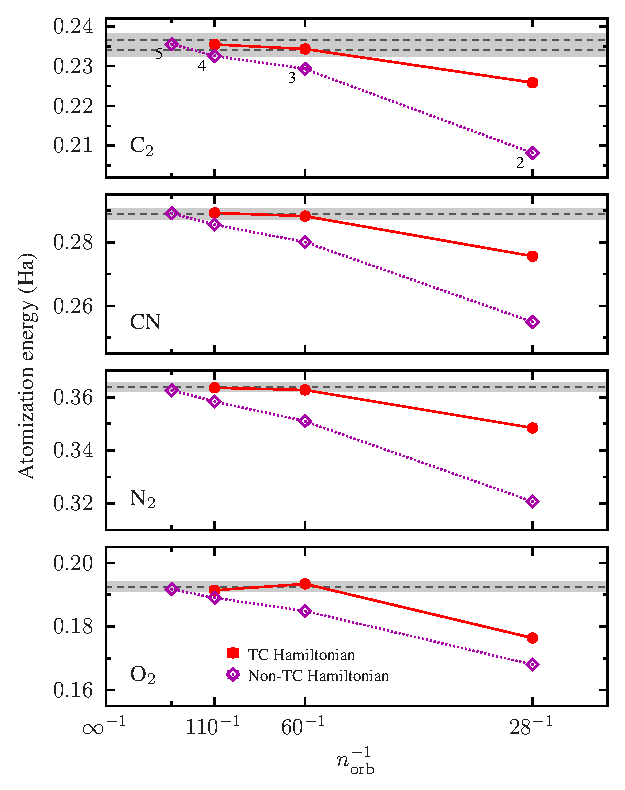
\includegraphics[width=0.8\textwidth]{figures/optimisation/Fig/bsdep-dimers-nontc}
    \caption{
      Atomisation energy of the C$_2$, CN, N$_2$, and O$_2$ molecules
      obtained with FCIQMC and TC-FCIQMC as a function of the
      reciprocal of the number of molecular orbitals using the
      \vxz{X} family of basis sets.
      %
      Points in the top panel are annotated with the basis set
      cardinal number $X$.
      %
      The shaded areas represent $\pm 1$ kcal/mol around the
      theoretical estimate of the non-relativistic atomisation energy
      of reference \citenum{fellerSurvey2008}; the distinct
      estimate of reference \citenum{bytautasCorrelation2005} is also
      shown for C$_2$.
    }
    \label{fig:bsdep-dimers-nontc}
  \end{center}
\end{figure}

As with the total energies, we find that the TC atomisation energies converge much faster with respect to basis-set size compared to the non-TC calculations. In fact, the TC results are already chemically accurate at the \vtz basis-set level, matching accuracy of \vxz{5} non-TC results. The application of the TC method to quantum chemical methods in
general could be presumed to be problematic because any theoretical
guarantee of cancellation of errors in energy differences disappears
with the introduction of separately-optimized Jastrow factors for each
system.
%
However, the fact that in our results the relative energy converges at
smaller basis-set sizes than the total energy implies that substantial
error cancellation is at play in practice.

\section{Conclusion and Outlook}

In this chapter, we presented a new method to optimise flexible Jastrow factors of a form common in continuum QMC methods for applications to TC. We tested these within the TC-FCIQMC framework. Minimising the variance of the reference energy is shown to be especially good for the TC method, since it maximises the single-reference character of the CI wave function.

These results show that this workflow can provide remarkably accurate total and relative energies, with relative energies at \vtz rivalling non-TC results at \vxz{5}. These results also provide better energy estimates compared to other promising methods, such as neural-network based trial wave functions.\supercite{pfauInitio2020,hermannDeepneuralnetwork2020}

Future work on this topic have focused on technical advancements and efficient approximations for dealing with the three-body integrals.

\subsection{The xTC Approximation}

One particularly significant refinement of this method is the so-called \gls{xTC} approximation,\supercite{christlmaierXTC2023} wherein upon neglecting explicit three-body contributions, the remaining three-body terms are ``folded'' into the remaining lower-order terms.

The Hamiltonian is normal-ordered with respect to $\Phi$ (where $\Psi=\e^J\Phi$, with $\Phi$ being the HF determinant in this chapter)\supercite{kutzelniggNormal1997,kutzelniggCumulant1999}

\begin{equation}
    H_N = \htc - \bra{\Phi}\htc\ket\Phi = F_N + V_N + L_N
\end{equation}
where the one-, two-, and three-body operators are (using Einstein summation)
\begin{align}
F_N =& [h_q^p + (U_{qs}^{pr}-U_{sq}^{pr})\gamma_s^r \\
&- \frac 12 (L_{qsu}^{prt} - L_{qus}^{prt}-L_{usq}^{prt})\gamma_{us}^{rt}]
\tilde a_q^p, \\
V_N =& \frac 12[U_{qs}^{pr} - (L_{qsu}^{prt} - L_{qus}^{prt}-L_{usq}^{prt})]\tilde a_{qs}^{pr}, \\
L_N =& \frac 16L_{qsu}^{prt}\tilde a_{qsu}^{prt}
\end{align}
and $U=V-K$, $\tilde a_{p\dots}^{q\dots}$ are the normal-ordered
excitation operators, and $\gamma_{p\dots}^{q\dots}=\bra\Phi a_{p\dots}^{q\dots}\ket\Phi$ are the density matrices.

Ignoring the three-body terms $L_N$ leads to an improved scaling with respect to basis set size while directly contracting intermediates to the lower-body corrections obviates the necessity to calculate $L$ and results in excellent energy agreement.\supercite{christlmaierXTC2023} Once the integrals are calculated, $\htc$ has, like $\hat H$, at most two-body interactions and therefore needs storage for four indices (albeit we no longer have Hermiticity). This means that calculations done on these integrals (in principle) are not much more expensive than the conventional non-TC calculations.

\label{sec:xtc}

% optimization paper
% different objective functions for optimizing the Jastrow factor
% "hat" functions
% no-3-body approximation (performance benchmarking)
% xTC approximation

% ch 5
\chapter{The Transcorrelated Method for Multireference Problems}
\label{chap:binding}

This chapter is based in large part on the following upcoming publication:\\
\fullcite{haupt_sizeconsistent}

Images have been reused from this paper (with permission).

\section{Introduction}

In this chapter, we apply the new framework for the transcorrated method described in chapter \ref{chap:opt} to problems of multireference character and find these methods may yield non-physical results. We propose an updated workflow wherein we use conventional post-Hartree-Fock methods as input to Jastrow optimisation for TC-FCIQMC. Results suggest size-consistent results and rapid basis set convergence compared to conventional methods, with the binding curve of N$_2$ at \avtz being within chemical accuracy of experiment.

\section{Motivation}

A popular ``stress test'' for quantum chemistry methods is the binding curve of N$_2$. Highly accurate experimental results\supercite{leroyAccurate2006} exist to recreate the curve, allowing for a useful benchmark. At equilibrium, this system is essentially single reference in character, but as the bond is stretched, the system becomes strongly multireference, making it particularly challenging for many methods. As an example, we might consider standard \gls{CCSD}, which is a single-reference method, compared to FCIQMC which (within stochastic error) is exact. Figure \ref{fig:ccsd-vs-fciqmc-n2} shows the binding curve of N$_2$ with CCSD compared to FCIQMC, using \avtz. We see that CCSD is not stable at large bond lengths.

\begin{figure}[htbp]
    \centering
    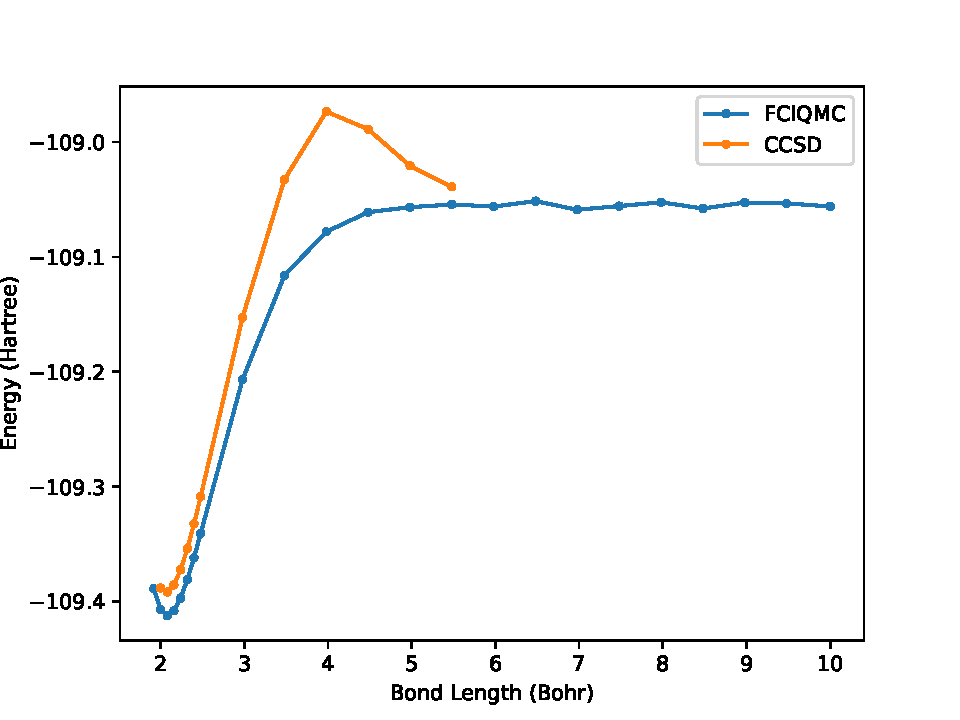
\includegraphics[width=0.8\textwidth]{figures/binding/N2_avtz_nontc}
    \caption{The binding curve for N$_2$ with the \avdz basis set. CCSD starts to decrease near 4 Bohr, which is nonphysical, whereas FCIQMC provides a more accurate curve. FCIQMC was done with 30 million walkers and HF-projected energy. The nonsmooth points in the dissociated region is due to stochastic error, and could be resolved with more walkers and a better trial wave function. CCSD did not converge at bond lengths larger than those shown.}
    \label{fig:ccsd-vs-fciqmc-n2}
\end{figure}

To see how well TC fares against such problems, consider the methodology outlined in chapter \ref{chap:opt}. We again use the same Jastrow factor as in equation \ref{eq:jastrow},
\begin{equation}
    \label{eq:jastrow-again}
    J = \sum_{i<j}^Nv(r_{ij}) + \sum_i^N\sum_I^{N_A}\chi(r_{iI}) + \sum_{i<j}^N\sum_I^{N_A}f(r_{ij}, r_{iI}, r_{jI}),
\end{equation}
with
\begin{equation}
    \label{eq:dtn-jastrow-ee-2}
    v(r_{ij})    = t(r_{ij},L_v)
                    \sum_{k} a_k r_{ij}^k ,
\end{equation}
\begin{equation}
    \label{eq:dtn-jastrow-en-2}
    \chi(r_{iI}) = t(r_{iI},L_\chi)
    \sum_{k} b_k r_{iI}^k ,
\end{equation}
\begin{equation}
    \label{eq:dtn-jastrow-een-2}
    f(r_{ij}, r_{i}, r_{j}) = t(r_{iI},L_f) t(r_{jI},L_f)
    \sum_{k,l,m} c_{klm}
    r_{ij}^k r_{iI}^l r_{jI}^m ,
\end{equation}
and the same cutoff functions $t(r,L) = (1-r/L)^3
\Theta(r-L)$. We also use the same objective function,
\begin{equation}
    \label{eq:varref-hf}
    \sigma_\mathrm{ref}^2 = \sum_{I\neq \mathrm{HF}}\bra{D_I}\htc\ket{D_\mathrm{HF}},
\end{equation}
Using this workflow with the xTC approximation, we calculate points along the binding curve of N$_2$, and find a non-physical ``dip'', as shown in figure \ref{fig:binding-dip}, similar to what CCSD exhibits in figure \ref{fig:ccsd-vs-fciqmc-n2}, albeit much more subtle.

\begin{figure}[htbp]
    \centering
    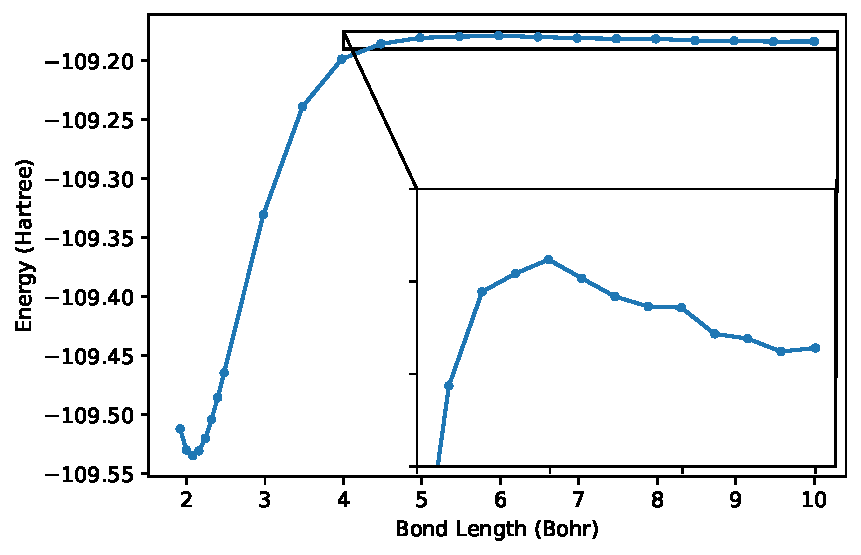
\includegraphics[width=0.8\textwidth]{figures/binding/inset_nontcfciqmc}
    \caption{The xTC-FCIQMC binding curve for N$_2$ with the \avtz basis set. While much smaller than that in figure \ref{fig:ccsd-vs-fciqmc-n2}, a non-physical dip is still present. This is apparent when zooming in on the curve, as shown in the inset.}
    \label{fig:binding-dip}
\end{figure}

This result has been verified for a few points with full TC (that is, with no approximations), which rules out xTC as the issue. Since the post-Hartree-Fock treatment was essentially at the FCI level, this implies that there is something wrong with the calculation of the Jastrow factors themselves. That is, our Hamiltonian is already ``corrupted'' before we even start the post-HF calculation.


\section{Resolving the Problem}

Based on the discussion in the previous section, it is likely that the transcorrelated workflow suffers from a single-reference bias. Indeed, the clear culprit is the Slater-Jastrow ansatz
\begin{equation}
    \label{eq:slater-jastrow}
    \Psi_\mathrm{SJ} = \e^J\Phi_\mathrm{HF},
\end{equation}
which affects the Jastrow optimisation and in turn the TC Hamiltonian $\htc = e^{-J}\hat H\e^J$.

We modify equation \ref{eq:slater-jastrow} to optimise for a multireference expansion,
\begin{equation}
    \label{eq:general-slater-jastrow}
    \Psi = \e^J\Phi_0
\end{equation}
where $\ket{\Phi_0}=\sum_I\ket{D_I}$. In practice, this modification results in two key changes in the workflow:
\begin{itemize}
    \item The objective function used during the VMC optimisation, equation \ref{eq:varref-hf}, needs to reflect the multireference ansatz. In particular, it will need to be changed to
    \begin{equation}
        \label{eq:varref-md}
        \sigma_\mathrm{ref}^2 = \sum_{I}\bra{D_I}\htc\ket{\Phi_0} - \bra{\Phi_0}\htc\ket{\Phi_0},
    \end{equation}
    which is evaluated in VMC by sampling
    \begin{equation}
        S_\mathrm{ref}^2 =
          \frac 1 {n_\mathrm{opt}-1}
          \sum_{n=1}^{n_\mathrm{opt}}
            \left| \frac {\hat H({\bm R}_n) \Psi({\bm R}_n)}
                         {\Psi({\bm R}_n)} - {\bar E}_\mathrm{ref}
            \right|^2.
    \end{equation}
    \item The density matrices used for xTC during integration must reflect this change as well. In particular, $\gamma_{p\dots}^{q\dots}=\bra{\Phi_0} a_{p\dots}^{q\dots}\ket{\Phi_0}$ in the equations in section \ref{sec:xtc}.
\end{itemize}

\subsection{Size Consistency}

One possible concern when studying problems like dissociation is that the method be size consistent. It is worth noting that one of the earliest Jastrow factors used for TC\supercite{boysCalculation1969} as well as in more recent work\supercite{cohenSimilarity2019} is given by
\begin{equation}
\label{eq:boyshandyjastrow}
J = \sum_{i<j} u(\bm r_i, \bm r_j)
\end{equation}
where
\begin{equation}
u(\bm r_i, \bm r_j) = \sum_{l,m,n}^{m+n+o\leq 6} c_{lmn}(\bar r_{iM}^m\bar r_{jN}^n+\bar r_{jM}^m\bar r_{iN}^n)\bar r_{ij}^l
\end{equation}
and $\bar r = r/(1+r)$.
However, notice that for $l=0$ and $n,m>0$, we can have non-vanishing gradients of $u$ for arbitrary distances between $N$ and $M$, and hence for systems $A$ and $B$ arbitrarily far apart we do not necessarily have
\begin{equation}
\label{eq:size-consistency}
e^{J_{A+B}}\ket{\Phi_{A+B}} = e^{J_0}(e^{J_{A}}\ket{\Phi_{A}})(e^{J_{B}}\ket{\Phi_{B}}),
\end{equation}
as $J_A$ will still act on system $B$, and vice versa. Here, $J_0$ is the electron-electron part of the Jastrow factor, $J_A$ the part involving nuclei in system $A$, and $J_B$ terms involving nuclei in system $B$.

In contrast to these previous works, our Jastrow ansatz, equation \ref{eq:jastrow-again}, first presented by Drummond, Towler and Needs,\supercite{drummondJastrow2004} vanishes when systems $A$ and $B$ are far apart due to the presence of the cutoff functions. Therefore, our Jastrow factor form does not suffer from this problem.

We must also ensure size consistency in our optimisation procedure. Assuming $\Phi_0$ is itself size consistent, it follows that for the given $J$, for non-interacting systems $A$ and $B$, the objective function, equation \ref{eq:varref-md}, $\sigma_\mathrm{ref}^2(A+B) = \sigma_\mathrm{ref}^2(A) + \sigma_\mathrm{ref}^2(B)$, where $\sigma_\mathrm{ref}^2(A)$ is the objective function for system $A$, and similarly for $B$. Hence, the parameters of the Jastrow factor should converge to the same values when treated as a non-interacting composite system as they would when treated as individual systems. Hence, our updated workflow is size consistent.

\subsection{Choices for Multireference Ansatzes}

We are now faced with the question of which choice of $\Phi_0$ is best. We present here three choices, and discuss their relative merits:
\begin{itemize}
    \item Using a FCIQMC wavefunction ansatz for $\Phi_0$. This is the most accurate one might get to the true solution, being essentially exact, but it is also computationally prohibitive for large systems. However, it is the most ``fool-proof'' proof-of-concept choice, can be treated as a blackbox (no need to choose an active space), and we might simply end the calculation early to get the most important components of the CI vector. In this chapter, we use a ``snapshot'' of the wave function at the end of a non-TC-FCIQMC calculation, and use the associated 1RDM calculated by the ``replica trick'' presented in section \ref{sec:fciqmc_rdm}. In this chapter, since our TC calculation is xTC-FCIQMC, using FCIQMC as the ansatz for $\Phi_0$ might be dubbed ``circular'' and actually does not worsen the computational scaling of the methodology. Of course, if we choose to use e.g. xTC-DCSD as our TC method, then the computational bottleneck is non-TC-FCIQMC, before we even begin transcorrelation.
    \item Using a CASSCF wavefunction ansatz for $\Phi_0$. In this method, the orbitals are also modified. It is a compromise compared to the FCIQMC approach, though still quite costly, is not a blackbox method, and a greater percentage of the wavefunction might be stored in the CI vector (since only a smaller subset of the orbitals are considered).
    \item Using a CASCI wavefunction ansatz for $\Phi_0$. Of the methods presented here, this is the least costly while still potentially capturing much of the static correlation needed and being relatively blackbox.\supercite{levineCAS2021} This is probably the most realistic choice for large-scale problems.
\end{itemize}

\section{Trial Wavefunctions in TC-FCIQMC}
\begingroup
\def\trial {\Phi_\mathrm{trial}}
\def\evec {\Phi_\mathrm{FCIQMC}}
Another challenge when studying multireference problems with FCIQMC is noise in the projected energy. Here we generalise the discussion on trial wavefunctions presented in section \ref{sec:fciqmc_energy_estimators}.

Consider a TC-FCIQMC calculation, where we wish to solve for the eigenvalue of the ground state $\Phi$ for the TC Hamiltonian $\htc$. Conventionally, the projected energy can be written
\begin{equation}
    E_\mathrm{proj} = \frac{\bra\trial\htc\ket\evec}{\braket{\trial}{\evec}}
\end{equation}
where $\ket\evec$ is the estimate of the wave function according to the FCIQMC algorithm, and $\ket\trial$ is the trial wave function. If we write $\ket\evec$ as a sum of the exact wave function $\ket{\Phi}$ plus some error $\ket\delta$, we have
\begin{align}
    E_\mathrm{proj} &= \frac{\bra\trial\htc\ket{\Phi+\delta}}{\braket{\trial}{\Phi+\delta}} \\
    &= \frac{E_0\braket{\trial}{\Phi}+\bra\trial\htc\ket{\delta}}{\braket{\trial}{\Phi}+\braket{\trial}{\delta}}
\end{align}
where $E_0$ is the exact ground-state energy.
If $\ket\trial$ is the left eigenvector, then $\bra\trial\htc\ket{\delta}=(\htc^\dag\ket\trial)^\dag\ket{\delta}=E_0\braket{\trial}{\delta}$, so
\begin{align}
    E_\mathrm{proj} &= \frac{E_0\braket{\trial}{\Phi}+E_0\braket{\trial}{\delta}}{\braket{\trial}{\Phi}+\braket{\trial}{\delta}}\\&=E_0\frac{\braket{\trial}{\Phi}+\braket{\trial}{\delta}}{\braket{\trial}{\Phi}+\braket{\trial}{\delta}}\\&=E_0,
\end{align}
i.e. if our trial wavefunction is the left eigenvector of $\htc$, then $E_\mathrm{proj}=E_0$.

In standard FCIQMC, we take the top $N_T$ determinants at some point of a calculation, form a subspace by constructing a $N_T\times N_T$ trial space $H_\mathrm{trial}$, diagonalise it exactly, and use the eigenvector as an approximation to the exact one, to be used as $\ket\trial$ in the calculation of the projected energy. As $H$ is Hermitian, taking the left or the right eigenvector is irrelevant. To get the left eigenvector in an equivalent way would involve doing a FCIQMC calculation on $\htc^\dag$, but this is costly and instead we find taking the left eigenvector of the subspace from $\htc$ to be a good approximation, as the two typically have similar top determinants. Moreover, this method gives the correct energy as long as the trial wavefunction has nonzero overlap with the true eigenvector, so even if our choice is not perfect, it will still give the correct answer, and likely with a smaller error compared to using the Hartree-Fock determinant.

\endgroup

As an example of the effectiveness of this approach,

\todo{present one example at dissociation showcasing the power of the methodology}

\section{Computational Details}

\section{Results}

\subsection{Binding Curves}
\todo{mention that we fix the binding curves}
\todo{also include a table about just ``how size-consistent'' the results actually are.}

\subsection{Excitation Energies}
\todo{mention can target the exact state(s) in question}

% \begin{table}[htbp]
%     \centering
%     \begin{tabular}{c|c|c|c}
%         Molecule & State & \avdz & \avtz & \avqz \\
%         \hline
%         N$_2$ & $^1\Sigma_g^+$ & & & \\
%     \end{tabular}
%     \caption{\todo{excitation energies for a couple of molecules, in mHa}}
%     \label{tbl:excitation-energies}
% \end{table}

\section{Conclusion and Outlook}
\todo{make sure to mention the cutoff analysis and constructing Jastrow factors from atomic Jastrow factors. Mention ECPs, since it's already been submitted...}
\todo{TC-CAS...}
\todo{self-consistent TC (i.e. feed back into itself)}

% size consistency/binding curve paper
% jastrow factor forms (DTN, BH)
% present problem that arises when trying to apply previous method to binding curves
% present how the problem exists even with xtc
% the sign problem in TC
% trial wave functions
% hydrogen chains? xTC-DCSD

% ch 6
\chapter{The PyTCHInt Library}
\label{chap:pytchint}

This chapter is based on the following software, to be released:\\
\fullcite{tchint}

The basis for how the library works is partially discussed in the following paper and its supplementary material: \\
\fullcite{cohenSimilarity2019}

\section{Introduction}

All transcorrelated matrix element calculations presented in this dissertation have been performed using the group's \tchint library or its Python extension, \pytchint. This library works by either producing transformed integral files, dubbed \fcidump files for four-index integrals,\todo{citation} or \tcdump files for the \gls{TC} six-index integrals. Note that since the \gls{TC} transformation is non-Hermitian, we do not have the same symmetries in these files as we do with conventional methods, or by interfacing with another program (such as \neci) or the Python interpreter (in the case of \pytchint).

As described in section \ref{sec:tc},
\begin{equation}
    \htc = \sum_{pq} h_q^p a_p^\dagger a_q
    + \frac{1}{2} \sum_{pqrs} \big(V_{rs}^{pq} - K_{rs}^{pq}\big)
    a_p^\dagger a_q^\dagger a_s a_r
    - \frac{1}{6} \sum_{pqrstu} L_{stu}^{pqr}
    a_p^\dagger a_q^\dagger a_r^\dagger a_u a_t a_s,
\end{equation}
where
\begin{equation}
\begin{split}
    h_q^p &= \bra{p}h\ket{q}, \\
    V_{rs}^{pq} &= \bra{p q } r_{12}^{-1} \ket{ r s}, \\
    K_{rs}^{pq} &= \bra{p q } \hat{K} \ket{ r s}, \\
    L_{stu}^{pqr} &= \bra{p q r } \hat{L} \ket{s t u}.
\end{split}
\end{equation}
$h_q^p$ and $V_{rs}^{pq}$ are the one- and two-body terms from the electronic Schr\"odinger equation, familiar from conventional methods. Therefore, the key quantities to be evaluated by \tchint are the non-Hermitian two-body integrals $K_{rs}^{pq}$ and the Hermitian three-body integrals $L_{stu}^{pqr}$.

Once these integrals are evaluated, as long as we take care about using the correct bra and ket (a detail not important for Hermitian problems), many different methodologies can be applied with these integrals, such as the frozen-core approximation,\todo{citation(s)} or \gls{xTC}.\todo{citation}

\section{Matrix Element Evaluation}
The matrix elements not present in conventional methods are $K_{rs}^{pq}$ and $L_{stu}^{pqr}$. For these, we integrate on a grid, typically Treutler-Ahlrichs integration grids,
\supercite{beckeMulticenter1988,treutlerEfficient1995} which are atom-centred grids commonly used in density functional theory. These grids are obtained via \pyscf.

The two-electron matrix elements we need to evaluate are:
\begin{align}
    K_{rs}^{pq(1)} &= \bra{pq}\nabla_1u(\bm r_1, \bm r_2)\cdot\nabla_1\ket{rs}\\
    K_{rs}^{pq(2)} &= \bra{pq}\nabla_1^2u(\bm r_1, \bm r_2)\ket{rs}\\
    K_{rs}^{pq(3)} &= \bra{pq}(\nabla_1u(\bm r_1, \bm r_2))^2\ket{rs}.
\end{align}
Discretising on a grid of $N_\mathrm{grid}$ points with weights $w$, we have
\begin{equation}
    K_{rs}^{pq(1)} = \sum_{mn}^{N_\mathrm{grid}}
    \phi_p(\bm r_m)\nabla_{\bm r_m}\phi_r(\bm r_m)\cdot \nabla_{\bm r_m}u(\bm r_m, \bm r_n)\phi_q(\bm r_n)\phi_s(\bm r_n)w(\bm r_m)w(\bm r_n).
\end{equation}
Naive integration of this value yields $\mathcal{O}(N_\mathrm{grid}^2M^4)$ performance (where $M$ is the number of basis functions). However, we may improve this by first integrating over one coordinate and storing the intermediate value. Moreover, for $K_{rs}^{pq(2)}$, it is more efficient to integrate by parts. Therefore, for the full $K$ matrix, we calculate the intermediate value
\begin{align}
    X_s^q(\bm r_2) =& \int\d^3 r_1\ \nabla_1u(\bm r_1, \bm r_2)\cdot[\phi_p(\bm r_1) \nabla_1\phi_r(\bm r_1) - \phi_r(\bm r_1)
\nabla_1\phi_p(\bm r_1)]  \\
&+ \int\d^3 r_1\ \phi_p(\bm r_1)(\nabla u(\bm r_1, \bm r_2))^2 \phi_r(\bm r_1).
\end{align}
We can then obtain the $K$ matrix by
\begin{equation}
    K_{rs}^{pq} = \int\d^3 r_2\ \phi_q(\bm r_2)X_s^q(\bm r_2)\phi_s(\bm r_2)
\end{equation}
for a cost of $\mathcal{O}(N_\mathrm{grid}^2M^2+N_\mathrm{grid}M^4)$.

The three-body matrix,
\begin{equation}
    L^{pqr}_{stu} = \bra{pqr}\nabla_1u(\bm r_1, \bm r_2)\cdot \nabla u_1(\bm r_1, \bm r_3)\ket{stu}
\end{equation}
may similarly be resolved by calculating the intermediate value
\begin{equation}
    \bm Y_{qt}(\bm r_1) = \int\d^3 r_2\phi_q(\bm r_2)\nabla_1u(\bm r_1, \bm r_2)\phi_t(\bm r_2)
\end{equation}
to give
\begin{equation}
    L^{pqr}_{stu} = \int\d^3 r_1\ \phi_p(\bm r_1)\bm Y_{qt}(\bm r_1)\cdot\bm Y_{ru}(\bm r_1)\phi_s(\bm r_1).
\end{equation}

These integrations are simply parallelisable, and \tchint takes advantage of this by leveraging distributed memory with the \gls{MPI}\todo{citation} standard and the OpenMP\todo{citation} \gls{API}. Moreover, we take advantage of the fact that $L$ is Hermitian, substantially reducing storage requirements. We may also store $L$ sparsely since many elements are small, or use the \gls{xTC} approximation to bypass storing $L$ altogether and instead calculating modified four-index integrals and outputting a non-Hermitian \fcidump.

\section{Interface}

\tchint is predominantly written in Fortran, but most of the important interfacing subroutines (such as returning given matrix elements) have C bindings. This allows \tchint to be easily interfaced with other libraries, notably for \gls{TC}-\gls{FCIQMC} in \neci\supercite{gutherNECI2020} and \mseven.\supercite{andersonRobertanderson2024} By using this interface, these programs may be used to perform transcorrelated calculations, with all the features present in \tchint.

\tchint has also been given a Python interface called \pytchint by making use of the Cython language extension.\todo{citation} Cython features C-like performance with easy integration in Python to allow for interactive computing and interfacing with the vast scientific package ecosystem available in Python. Python is typically also easier for rapid prototyping, a crucial feature in the world of scientific research, while Cython provides efficiency and a comprehensive profiling toolset.

With \pytchint, a user might interactively work with transcorrelated integrals by first calculating them,
\begin{lstlisting}[language=Python,escapeinside={(*}{*)}]
import pytchint
options = pytchint.options.TcOptions(yaml_input="tchint.yml")
options.eval_mode_str = "xtc"
solver = pytchint.solver.Solver(options=options)
solver.run()
\end{lstlisting}
and then query individual matrix elements calculated via Slater-Condon rules with \texttt{solver.sltcnd} or return the variance of the reference with \texttt{solver.refconn}.

\subsection{Deterministic Optimisation}

One of the major motivations for developing the Python interface

\todo{mention it uses the interface for existing high-performing optimisation packages, rapid prototyping}

\section{Parallel Efficiency}

\todo{...}
As a benchmark, we consider the N$_2$ molecule at

AMD EPYC 9554 64-Core processors

Figure \ref{fig:parallel-performance} shows the elapsed

Fortran 468 seconds vs Python 465 seconds

\begin{figure}[htbp]
    \centering
    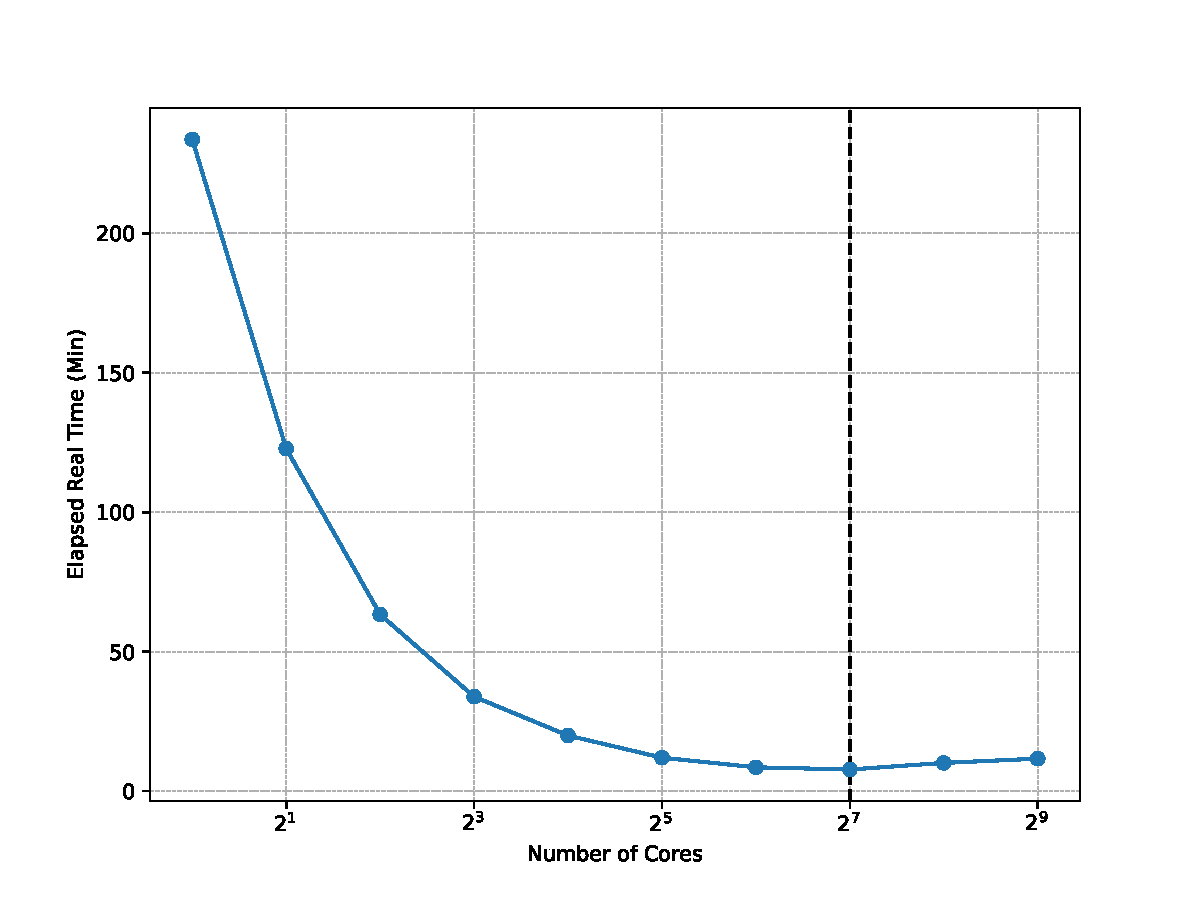
\includegraphics[width=0.8\textwidth]{figures/pytchint/ncore_walltime}
    \caption{\todo{\dots note logarithmic x axis}}
    \label{fig:parallel-performance}
\end{figure}

\todo{not really sure how I'll write this section, since I don't really have a performance metric to go up against}
\todo{parallel efficiency}
\todo{memory requirements, with vs without xTC vs no-3b -- mention already covered in optimisation chapter}
\todo{mention other smaller details, such as never calculating the L matrix during xTC}
\todo{pytchint vs tchint performance}
\todo{accuracy of full vs 3bera vs xtc}
\todo{mention use of BLAS routines}

\section{Conclusion and Outlook}
\todo{mention GPU acceleration, Python libraries, JAX (+ AD?), deterministic optimisation with universal Jastrow factors, interfacing with other QMC libraries, more studies with solids ...}

% the pytchint library
% library, integrals, how it works (see Aron's notes, paper)
% xtc implementation
% many options
% deterministic optimisation
% benchmarking?
% Python package

\chapter{Summary and Outlook}
  \label{chap:sumandout}
\todo{...}
\todo{brief review}
\todo{outlook: ECPs (if not already published), efficient deterministic optimisation, better understanding of the form of the Jastrow factor and other options, pytchint optimisation, larger molecules, solids, embedding, CUDA}

% solids, ecps, deterministic optimisation, tc-casscf, etc.
% focus on pytchint

\listoffigures
\listoftables
\printbibliography
\appendix
\chapter{Appendix (todo)}

\todo{Not sure what will be needed in appendices.}
% \section{sec}
% \subsection{subsec}
% \label{app:}

\chapter{Curriculum vitae}
  \label{Chap:CV}

  \section*{Education}
  \begin{small}
    \begin{tabular}{L{2.5cm}L{10cm}}
      \textbf{2020 -- 2025} & PhD student, Theoretical Chemistry\\
             & Max Planck Institute for Solid State Research, Stuttgart, Germany \\
             & \textbf{Thesis:} \thetitle \\
             & \textbf{Advisors:} Prof Ali Alavi \\
      \\
      \textbf{2014 -- 2019} & Bachelor of Science, Honours Physics and Mathematics, Minor in Computer Science\\
                  & University of British Columbia, Vancouver, Canada \\
             & \textbf{Thesis:}  Effects of Anisotropic Long-Range Hopping on Anderson Localization\\
             & \textbf{Advisor:} Prof Roman Krems \\
      \\
    \end{tabular}
  \end{small}

% \clearpage

\section*{Publications}
\begin{refsection}
\setmaxcitenames{10}

\begin{singlespace}
\begin{footnotesize}

\subsection*{First authored}
\begin{enumerate}[label=(\arabic*), itemindent=-0.5em]
    \item \todo{publications, I guess: optimization paper, binding curve paper, pytchint paper (likely with a "to be submitted")}
%   \item \fullcite*{..}
\end{enumerate}

\subsection*{Co-authored}
\begin{enumerate}[resume, label={(\arabic*)}, itemindent=-0.5em]
    \item \todo{publications, I guess: ECPs, 2nd row atoms, deterministic optimisation, spin-dependent Jastrows}
%   \item \fullcite*{...}
\end{enumerate}

\end{footnotesize}
\end{singlespace}

\end{refsection}
\end{document}
